\documentclass{article}
\usepackage[utf8]{inputenc}

% Standard math packages
\usepackage{amsmath}
\usepackage{amsthm}
\usepackage{amssymb}
\usepackage{amsfonts}

% Packages for images
\usepackage{tikz}

% Package for the layout
\usepackage{geometry}

% Title Page
\title{Calculus}
\author{Jonathan Parker}
\date{Last Updated on \today}

% Counters
\renewcommand*\contentsname{Table of Contents}

\newtheorem{theorem}{Theorem}[section]

\newtheorem{definition}{Definition}[section]

\newtheorem{note}{Note}[section]

\newcounter{example}[section]
\newenvironment{example}[1][]{\refstepcounter{example}\par\medskip
   \noindent \textbf{Example~\theexample. #1} \rmfamily}{\medskip}

\newcounter{exercise}[section]
\newenvironment{exercise}[1][]{\refstepcounter{exercise}\par\medskip
   \noindent \textbf{Exercise~\theexercise. #1} \rmfamily}{\medskip}
   
\newcounter{recall}[section]
\newenvironment{recall}[1][]{\refstepcounter{recall}\par\medskip
   \noindent \textbf{Recall~\therecall. #1} \rmfamily}{\medskip}
   
% Declarations
\DeclareMathOperator*{\arccot}{arccot}
\DeclareMathOperator*{\arcsec}{arcsec}
\DeclareMathOperator*{\arccsc}{arccsc}
   
% Removing indentations
\setlength{\parindent}{0pt}


\begin{document}

\maketitle
\tableofcontents

\newpage
\documentclass{article}
\usepackage[utf8]{inputenc}
\usepackage{amsmath}
\usepackage{amsthm}
\usepackage{amssymb}
\usepackage{geometry}
\usepackage{amsfonts} 

\title{Sequences of Numbers}
\author{Jonathan Parker}
\date{Last Updated on \today}

\renewcommand*\contentsname{Table of Contents}

\newtheorem{theorem}{Theorem}[section]

\newtheorem{definition}{Definition}[section]

\newtheorem{note}{Note}[section]

\newcounter{example}[section]
\newenvironment{example}[1][]{\refstepcounter{example}\par\medskip
   \noindent \textbf{Example~\theexample. #1} \rmfamily}{\medskip}

\newcounter{exercise}[section]
\newenvironment{exercise}[1][]{\refstepcounter{exercise}\par\medskip
   \noindent \textbf{Exercise~\theexercise. #1} \rmfamily}{\medskip}
   
\newcounter{recall}[section]
\newenvironment{recall}[1][]{\refstepcounter{recall}\par\medskip
   \noindent \textbf{Recall~\therecall. #1} \rmfamily}{\medskip}
   
\setlength{\parindent}{0pt}

\begin{document}


\maketitle
\tableofcontents

\newpage
\section{Introduction to Sequences of Numbers}\label{introduction_to_sequences_of_numbers}

\begin{definition}
A sequence of real numbers is a mapping
\begin{align*}
    f: \mathbb{N} \longrightarrow \mathbb{R}: f(n) \mapsto a_{n}
\end{align*}
We typically write the sequence in the following concise way:
\begin{align*}
    \{f(n)\}_{n=1}^{\infty} \hspace{20pt} \text{or} \hspace{20pt} \{a_{n}\}_{n=1}^{\infty}
\end{align*}
where $a_{n}$ is the real number function value at index $n$.
\end{definition}

\begin{example}
\begin{align*}
    &\Big\{\dfrac{1}{n}\Big\}_{n=1}^{\infty}\\[2ex]
    = \hspace{4pt} &\Big\{\dfrac{1}{1}, \hspace{4pt} \dfrac{1}{2}, \hspace{4pt} \dfrac{1}{3}, \hspace{4pt} \cdots \Big\}
\end{align*}
Here, $f(n) = \dfrac{1}{n}$ is the function definition from the natural numbers $\mathbb{N}$ to the real numbers $\mathbb{R}$.
\end{example}

\begin{exercise}
Write the $5^{\text{th}}$ term for the following sequence of real numbers:
\begin{align*}
    \Big\{\dfrac{n}{n+1}\Big\}_{n=1}^{\infty}
\end{align*}
\end{exercise}

\begin{exercise}
Write the first five terms for the following sequence of real numbers:
\begin{align*}
    \Big\{\dfrac{(-1)^{n}(n+1)}{3^{n}}\Big\}_{n=1}^{\infty}
\end{align*}
\end{exercise}

Sometimes, the domain is extended or attenuated a bit to accommodate the function definition.

\begin{exercise}
Write the first five terms for the following sequence of real numbers:
\begin{align*}
    \{\sqrt{n-10}\}_{n=10}^{\infty}
\end{align*}
\end{exercise}

\begin{exercise}
Write the first five terms for the following sequence of real numbers:
\begin{align*}
    \Big\{\cos{\Big(\dfrac{n\pi}{4}\Big)}\Big\}_{n=0}^{\infty}
\end{align*}
\end{exercise}

A tricky part of this concept is using a sequence's function values to determine the general formula.

\begin{example}
Let's take the following sequence of terms:
\begin{align*}
    \Big\{\dfrac{3}{5}, \hspace{4pt} -\dfrac{4}{25}, \hspace{4pt} \dfrac{5}{125}, \hspace{4pt} -\dfrac{6}{625}, \hspace{4pt} \dfrac{7}{3125}, \hspace{4pt} \cdots \Big\}
\end{align*}
Our job is to discover a pattern. Well, it seems every other term is negative. We know this can be established with the factor $(-1)^{n}$, but given that there are other factors we've yet to analyze thoroughly, it's not certain that this is a factor in our general expression for the sequence. It also seems the numerator begins at $3$ and increments by one unit as the sequence progresses. Given that the sequence begins at $n=3$, will our first term in the sequence be positive? We see $(-1)^{3}$ is negative. So, we fix this by adding or subtracting a $1$ from the power $n$. While it is not always the case that either adding or subtracting a $1$ will work, in this example, either approach will. So, we add a $1$, giving us $(-1)^{n+1}$ as a factor in our general sequence. Finally, the denominator seems to be some power of $5$ in each term of the sequence, and it seems those powers begin at $1$, which is equal to $3-2$. Checking the power in our second term, we have a power of $2$, which is equal to $4-2$. It seems our powers progress through the expression $n-2$, where $n$ is the index of the sequence. Thus, we have the following general expression for our sequence:
\begin{align*}
    \Big\{\dfrac{(-1)^{n+1}n}{5^{n-2}}\Big\}_{n=3}^{\infty}
\end{align*}
\end{example}

\begin{exercise}
Find the general expression of the sequence following the pattern:
\begin{align*}
    \Big\{1, \hspace{4pt} -\dfrac{2}{3}, \hspace{4pt} \dfrac{4}{9}, \hspace{4pt} -\dfrac{8}{27}, \hspace{4pt} \cdots \Big\}
\end{align*}
\end{exercise}

\newpage
\section{Limits of Sequences of Numbers}\label{limits_of_sequences_of_numbers}

\begin{definition}
A sequence $\{f(n)\}_{n=1}^{\infty}$ has a limit $L$, which we denote as 
\begin{align*}
    \lim_{n \longrightarrow \infty} f(n) = L\\[2ex]
    \text{if for all} \hspace{4pt} \epsilon > 0 \hspace{4pt} \text{there exists a natural number} \hspace{4pt} &N \hspace{4pt} \text{such that for all} \hspace{4pt} n \geq N \hspace{4pt} \text{we have}\\[2ex]
    \lvert f(n) - L \rvert < \epsilon
\end{align*}
Any sequence with a limit can be referred to as convergent.
\label{definition_limit_sequence_numbers}
\end{definition}

\begin{example}
$\lim_{n \longrightarrow \infty} \dfrac{1}{n} = 0$
\begin{proof}
Take $\epsilon = \dfrac{1}{k}$, where $k \in \mathbb{N}$ is arbitrary. Then by Definition \ref{definition_limit_sequence_numbers} we have
\begin{align*}
    &\Big\lvert \dfrac{1}{k+n} - 0 \Big\rvert\\[2ex]
    &= \Big\lvert \dfrac{1}{k+n} \Big\rvert\\[2ex]
    &< \dfrac{1}{k} = \epsilon, \hspace{4pt} \text{for all} \hspace{4pt} n \in \mathbb{N}
\end{align*}
\end{proof}
\label{limit_one_over_n}
\end{example}

\begin{theorem}
If $\{f(n)\}_{n=1}^{\infty}$ and $\{g(n)\}_{n=1}^{\infty}$ are convergent sequences, and if $c \in \mathbb{R}$, then
\begin{align*}
    &\lim_{n \longrightarrow \infty} (f(n) + g(n)) = \lim_{n \longrightarrow \infty} f(n) + \lim_{n \longrightarrow \infty} g(n) \\[2ex]
    &\lim_{n \longrightarrow \infty}(f(n) - g(n)) = \lim_{n \longrightarrow \infty} f(n) - \lim_{n \longrightarrow \infty} g(n)\\[2ex]
    &\lim_{n \longrightarrow \infty} cf(n) = c\lim_{n \longrightarrow \infty} f(n)\\[2ex]
    &\lim_{n \longrightarrow \infty} (f(n) \cdot g(n)) = \lim_{n \longrightarrow \infty} f(n) \cdot \lim_{n \longrightarrow \infty} g(n)\\[2ex]
    &\lim_{n \longrightarrow \infty}\dfrac{f(n)}{g(n)} = \dfrac{\lim_{n \longrightarrow \infty} f(n)}{\lim_{n \longrightarrow \infty} g(n)}, \hspace{4pt} \text{when} \hspace{4pt} \lim_{n \longrightarrow \infty} g(n) \neq 0\\[2ex]
    &\lim_{n \longrightarrow \infty} (f(n))^{p} = (\lim_{n \longrightarrow \infty} f(n))^{p}, \hspace{4pt} \text{where} \hspace{4pt} p > 0 \hspace{4pt} \text{and} \hspace{4pt} f(n) > 0\\[2ex]
    &\lim_{n \longrightarrow \infty} c = c
\end{align*}
\label{properties_limit_sequence_numbers}
\end{theorem}

Now that we have these result, we can use them to find limits of other sequences.

\begin{example}
$\lim_{n \longrightarrow \infty} \dfrac{n}{n+1} = 1$
\begin{proof}
We have a trick we can employ to find the above limit. By Example \ref{limit_one_over_n} and Theorem \ref{properties_limit_sequence_numbers},
\begin{align*}
    \dfrac{n}{n+1} &= 1 \cdot \dfrac{n}{n+1}
    = \dfrac{1/n}{1/n} \cdot \dfrac{n}{n+1}
    = \dfrac{(1/n) \cdot n}{(1/n) \cdot (n+1)}
    = \dfrac{1}{1 + (1/n)}\\[2ex]
    \Longrightarrow &\lim_{n \longrightarrow \infty} \dfrac{n}{n+1}
    = \lim_{n \longrightarrow \infty} \dfrac{1}{1+(1/n)}
    = \dfrac{\lim_{n \longrightarrow \infty}1}{\lim_{n \longrightarrow \infty}1 + \lim_{n \longrightarrow \infty}(1/n)}
    = \dfrac{1}{1 + 0} = 1
\end{align*}
\end{proof}
\end{example}

\begin{exercise}
Find the limit of 
\begin{align*}
    \Big\{\dfrac{n^{3}}{n^{3}+1}\Big\}_{n=1}^{\infty}
\end{align*}
\end{exercise}

\begin{exercise}
Find the limit of 
\begin{align*}
    \Big\{\dfrac{3+5n^{2}}{n+n^{2}}\Big\}_{n=1}^{\infty}
\end{align*}
\end{exercise}

\begin{exercise}
Find the limit of 
\begin{align*}
    \{e^{1/n}\}_{n=1}^{\infty}
\end{align*}
\end{exercise}

\begin{exercise}
Find the limit of
\begin{align*}
    \Big\{\tan\Big(\dfrac{2n\pi}{1+8n}\Big)\Big\}_{n=1}^{\infty}
\end{align*}
\end{exercise}

\begin{exercise}
Find the limit of
\begin{align*}
    \Big\{\sqrt{\dfrac{n+1}{9n+1}}\Big\}_{n=1}^{\infty}
\end{align*}
\end{exercise}

\begin{definition}
Take a sequence $\{f(n)\}_{n=1}^{\infty}$ 
\begin{align*}
    \text{If} \hspace{4pt} \lim_{n \longrightarrow \infty} f(n) &= \infty, \hspace{4pt} \text{then}\\[2ex]
    \text{for all} \hspace{4pt} N \in \mathbb{N}, \hspace{4pt} \text{there exists an} \hspace{4pt} M \in \mathbb{N} \hspace{4pt} &\text{such that for all} \hspace{4pt} n > M \hspace{4pt} \text{we have} \hspace{4pt} f(n) > N.
\end{align*}
\begin{align*}
    \text{If} \hspace{4pt} \lim_{n \longrightarrow \infty} f(n) &= -\infty, \hspace{4pt} \text{then}\\[2ex]
    \text{for all} \hspace{4pt} N \in \mathbb{N}, \hspace{4pt} \text{there exists an} \hspace{4pt} M \in \mathbb{N} \hspace{4pt} &\text{such that for all} \hspace{4pt} n > M \hspace{4pt} \text{we have} \hspace{4pt} f(n) < -N.
\end{align*}
Any sequence with an infinite limit is said to be divergent.
\label{definition_infinite_limit_sequence}
\end{definition}

\begin{example}
Take $\{n\}_{n=1}^{\infty}$. Clearly, as $n \longrightarrow \infty$, the sequence of function values push to infinity.
\end{example}

\begin{exercise}
Show the sequence $\Big\{\dfrac{n^{3}}{n+1}\Big\}_{n=1}^{\infty}$ has an infinite limit. 
\end{exercise}

\begin{exercise}
Show the sequence $\Big\{\dfrac{n!}{2^{n}}\Big\}_{n=1}^{\infty}$ has an infinite limit. 
\end{exercise}

\begin{theorem}
A sequence of numbers can have at most one limit.
\label{limit_uniqueness}
\end{theorem}

\begin{note}
Any sequence that does not converge to a single, finite value is considered divergent.
\end{note}

\begin{exercise}
Find the general expression of the divergent sequence following the pattern:
\begin{align*}
    \{5, \hspace{4pt} 1, \hspace{4pt} 5, \hspace{4pt} 1, \hspace{4pt} 5, \hspace{4pt} 1, \hspace{4pt} \cdots\}
\end{align*}
\end{exercise}

\begin{exercise}
Find the general expression of the divergent sequence following the pattern:
\begin{align*}
    \{2, \hspace{4pt} 7, \hspace{4pt} 12, \hspace{4pt} 17, \hspace{4pt} \cdots\}
\end{align*}
\end{exercise}

\begin{exercise}
Determine whether the sequence defined by the following is convergent or divergent:
\begin{align*}
    f(1) = 1 \hspace{20pt} f(n) = 4 - f(n-1), \hspace{20pt} n \geq 1
\end{align*}
\end{exercise}

\begin{exercise}
Determine whether the sequence defined by the following is convergent or divergent:
\begin{align*}
    f(1) = 2 \hspace{20pt} f(n) = 4 - f(n-1), \hspace{20pt} n \geq 1
\end{align*}
\end{exercise}

\begin{recall}
For all $a, b \in \mathbb{R}$, we have
\begin{align*}
    \Big\lvert \lvert a \rvert - \lvert b \rvert \Big\rvert &\leq \lvert a - b \rvert \\[2ex]
    \lvert a + b \rvert &\leq \lvert a \rvert + \lvert b \rvert
\end{align*}
\label{triangle_inequality}
\end{recall}

\begin{theorem}
Let $\{f(n)\}_{n=1}^{\infty}, \hspace{4pt} \{g(n)\}_{n=1}^{\infty}$ and $\{h(n)\}_{n=1}^{\infty}$ be sequences. If
\begin{align*}
    \text{If} \hspace{4pt} f(n)\leq g(n)\leq h(n) \hspace{4pt} \text{for all} \hspace{4pt} n \in \mathbb{N} \hspace{20pt}
    & \text{and if}  \hspace{20pt} \lim_{n \longrightarrow \infty} f(n) = \lim_{n \longrightarrow \infty} g(n) = L \\[2ex]
    & \text{then} \hspace{4pt} \lim_{n \longrightarrow \infty} h(n) = L 
\end{align*}
\label{squeeze_theorem}
\end{theorem}

\begin{exercise}
Show the following two different ways:
\begin{itemize}
    \item [1.] Using the triangle inequality from Recall \ref{triangle_inequality}
    \item [2.] Using Theorem \ref{squeeze_theorem}
\end{itemize}
\begin{align*}
    \lim_{n \longrightarrow \infty} \dfrac{(-1)^{n-1}n}{n^{2}+1} = 0
\end{align*}
\end{exercise}

\begin{exercise}
Prove the following theorem two different ways:
\begin{itemize}
    \item [1.] Using the triangle inequality from Recall \ref{triangle_inequality}
    \item [2.] Using Theorem \ref{squeeze_theorem}
\end{itemize}
\begin{align*}
    \text{If} \hspace{4pt} \lim_{n \longrightarrow \infty} \lvert f(n) \rvert = L \hspace{20pt} \text{then} \hspace{20pt} \lim_{n \longrightarrow \infty} f(n) = L
\end{align*}
\end{exercise}

\begin{exercise}
Use Theorem \ref{squeeze_theorem} to find the limit of the following sequence:
\begin{align*}
    \Big\{\dfrac{\sin(n)}{n}\Big\}_{n=1}^{\infty}
\end{align*}
\end{exercise}

\begin{exercise}
Use Theorem \ref{squeeze_theorem} to find the limit of the following sequence:
\begin{align*}
    \Big\{\dfrac{\cos^{2}(n)}{2^{n}}\Big\}_{n=1}^{\infty}
\end{align*}
\end{exercise}

\begin{exercise}
Use Theorem \ref{squeeze_theorem} to find the limit of the following sequence:
\begin{align*}
    \Big\{\dfrac{\sin(2n)}{1+\sqrt{n}}\Big\}_{n=1}^{\infty}
\end{align*}
\end{exercise}

\begin{exercise}
Find the limit of the following sequence:
\begin{align*}
    \Big\{\dfrac{n!}{2^{n}}\Big\}_{n=1}^{\infty}
\end{align*}
\end{exercise}

\begin{exercise}
Find the limit of the following sequence:
\begin{align*}
    \Big\{\dfrac{(-3)^{2}}{n!}\Big\}_{n=1}^{\infty}
\end{align*}
\end{exercise}

\end{document}


\newpage
\section{Limits of Functions}

\begin{definition}
We say $f$ as a function of $x$ has a limit $L$ at $c \in \mathbb{R}$, denoted by
\begin{align*}
    &\lim_{x \longrightarrow c} f(x) = L \hspace{4pt} \text{if} \hspace{20pt} &&\text{for all} \hspace{4pt} \epsilon > 0, \hspace{4pt} \text{there exists a} \hspace{4pt} \delta > 0 \hspace{4pt} \text{such that}\\[2ex]
    &\text{for all} \hspace{4pt} x \in \text{Dom($f$)} \hspace{4pt} \text{satisfying} \hspace{4pt} \lvert x - c \rvert < \delta &&\text{we have} \hspace{4pt} \lvert f(x) - L \rvert < \epsilon
\end{align*}
\end{definition}

\begin{example}
Below is a visual of how this $\epsilon - \delta$ interplay occurs. In general, if $L \in \mathbb{R}$ is the limit of $f$ at $c \in \mathbb{R}$, then for an arbitrarily small, open interval $(L-\epsilon, L+\epsilon)$ with center $L$, there is an open interval $(c-\delta, c+\delta)$ with center $c$ containing members $x \in$ Dom($f$). With this specific example, $c=1/2$. For any $x \in$ Dom($f$) satisfying 
\begin{align*}
    \Big\lvert x - \dfrac{1}{2} \Big\rvert < \delta \hspace{20pt} \text{we have} \hspace{20pt} \lvert f(x) - L \rvert = \lvert \sin(x) - L \rvert < \epsilon \hspace{20pt} \Longleftrightarrow \hspace{20pt} \lim_{x \longrightarrow 1/2} \sin(x) = L
\end{align*}
which is equivalent to the following: For any $x \in$ Dom($f$) satisfying
\begin{align*}
    x \in \Big(\dfrac{1}{2} - \delta, \dfrac{1}{2} + \delta\Big) \hspace{20pt} \text{we have} \hspace{4pt} f(x) \in (L - \epsilon, L + \epsilon)
\end{align*}

\resizebox{30em}{30em}{%
\begin{tikzpicture}[scale=\textwidth/4.2cm]
    % title and axes
    \node at (0.7, 1.1) {\tiny$f(x)=\sin x \hspace{4pt} x \in \Big[0, \dfrac{1}{2}\Big) \cup \Big(\dfrac{1}{2}, 1 \Big]$};
    \draw (0, 0) -- (1, 0)
        node[right] {\tiny$x$};
    \draw (0, 0) -- (0, 1)
        node[above] {\tiny$f(x)$};
    % ----------------------------------
    % range boundaries lower
    \draw[dotted] (0, {sin(0.45 r)}) -- (0.6, {sin(0.45 r)});
    \node[] at (-0.15, {sin(0.45 r)}) {\tiny$L-\epsilon$};
    \node [rotate=90] at (0, {sin(0.45 r)}) {\tiny(};
    % range boundaries upper
    \draw[dotted] (0, {sin(0.55 r)}) -- (0.6, {sin(0.55 r)});
    \node[] at (-0.15, {sin(0.55 r)}) {\tiny$L+\epsilon$};
    \node [rotate=-90] at (0, {sin(0.55 r)}) {\tiny(};
    % ----------------------------------
    % domain boundaries lower
    \draw[dotted] (0.47, 0) -- (0.47, {sin(0.6 r)});
    \node [rotate=45] at (0.35, -0.15) {\tiny$\dfrac{1}{2}-\delta$ $\longrightarrow$};
    \node [] at (0.47, 0) {\tiny(};
    % domain boundaries upper
    \draw[dotted] (0.53, 0) -- (0.53, {sin(0.6 r)});
    \node [rotate=-45] at (0.65, -0.15) {\tiny$\longleftarrow$ \tiny$\dfrac{1}{2}+\delta$};
    \node [] at (0.53, 0) {\tiny)};
    % ----------------------------------
    % graph
    \draw[blue] plot[smooth] file {limits_of_functions/python_generated_tables/sine_0_1_piece_0.table};
    \draw[blue] plot[smooth] file {limits_of_functions/python_generated_tables/sine_0_1_piece_1.table};
    \draw[blue, fill=white] (0.5,{sin(0.5 r)}) circle (.25mm);
\end{tikzpicture}
}
\end{example}

\begin{exercise}
Find the following:
\begin{align*}
    \lim_{x \longrightarrow 1/2} \sin(x) \hspace{20pt} x \in [0, 1]
\end{align*}
\end{exercise}

\begin{theorem}
If $f(x) = x, \hspace{4pt} x \in \mathbb{R}$, then $\lim_{x \longrightarrow c} f(x)$ exists for all $c \in \mathbb{R}$. Because $f$ is defined on the entire real line, we have 
\begin{align*}
    \lim_{x \longrightarrow c} f(x) = f(c) = c
\end{align*}
\label{limit_identity_function}
\end{theorem}

\begin{theorem}
Suppose $c \in \mathbb{R}$ and suppose 
\begin{align*}
    \lim_{x \longrightarrow a} f(x) \hspace{20pt} \text{and} \hspace{20pt} \lim_{x \longrightarrow a} g(x)
\end{align*}
both exist. Then we have
\begin{align*}
    &\lim_{x \longrightarrow a} [f(x) + g(x)] = \lim_{x \longrightarrow a} f(x) + \lim_{x \longrightarrow a} g(x)\\[2ex]
    &\lim_{x \longrightarrow a} [f(x) - g(x)] = \lim_{x \longrightarrow a} f(x) - \lim_{x \longrightarrow a} g(x)\\[2ex]
    &\lim_{x \longrightarrow a} [c \cdot f(x)] = c \cdot \lim_{x \longrightarrow a} f(x)\\[2ex]
    &\lim_{x \longrightarrow a} [f(x) \cdot g(x)] = \lim_{x \longrightarrow a} f(x) \cdot \lim_{x \longrightarrow a} g(x)\\[2ex]
    &\lim_{x \longrightarrow a} \dfrac{f(x)}{g(x)} = \dfrac{\lim_{x \longrightarrow a} f(x)}{\lim_{x \longrightarrow a} g(x)} \hspace{20pt} \text{when} \hspace{4pt} \lim_{x \longrightarrow a} g(x) \neq 0
\end{align*}
\label{properties_limit_functions}
\end{theorem}

\begin{example}
Here is another example, taking the mathematical approach, using Theorems \ref{limit_identity_function}, \ref{properties_limit_functions}, to find the limit,
\begin{align*}
    \lim_{x \longrightarrow 1} \dfrac{x-1}{x^{2} - 1} = \lim_{x \longrightarrow 1} \dfrac{x-1}{(x-1)(x+1)} = \lim_{x \longrightarrow 1} \dfrac{1}{(x+1)} = \dfrac{1}{(1+1)} = \dfrac{1}{2}
\end{align*}

\resizebox{30em}{30em}{%
\begin{tikzpicture}[scale=\textwidth/6.2cm]
    % title and axes
    \node at (1.5, 2.1) {\tiny$f(x)=\dfrac{x-1}{x^{2}-1} \hspace{4pt} x \in \Big[\dfrac{1}{2}, 1\Big) \cup (1, 2]$};
    \draw (-0.5, 0) -- (2, 0)
        node[right] {\tiny$x$};
    \draw (0, 0) -- (0, 2)
        node[above] {\tiny$f(x)$};
    % ----------------------------------
    % range boundaries lower
    \draw[dotted] (0, 0.45) -- (1.05, 0.45);
    \node[rotate=45] at (-0.20, 0.28) {\tiny$\dfrac{1}{2}-\epsilon \longrightarrow$};
    \node [rotate=90] at (0, 0.45) {\tiny(};
    % range boundaries upper
    \draw[dotted] (0, 0.55) -- (1.05, 0.55);
    \node[rotate=-45] at (-0.20, 0.72) {\tiny$\dfrac{1}{2}+\epsilon \longrightarrow$};
    \node [rotate=-90] at (0, 0.55) {\tiny(};
    % ----------------------------------
    % domain boundaries lower
    \draw[dotted] (0.95, 0) -- (0.95, 0.55);
    \node [rotate=45] at (0.75, -0.2) {\tiny$1-\delta$ $\longrightarrow$};
    \node [] at (0.95, 0) {\tiny(};
    % domain boundaries upper
    \draw[dotted] (1.05, 0) -- (1.05, 0.55);
    \node [rotate=-45] at (1.25, -0.2) {\tiny$\longleftarrow$ \tiny$1+\delta$};
    \node [] at (1.05, 0) {\tiny)};
    % ----------------------------------
    % graph
    \draw[blue] plot[smooth] file {limits_of_functions/python_generated_tables/rational_neg1half_2_piece_0.table};
    \draw[blue] plot[smooth] file {limits_of_functions/python_generated_tables/rational_neg1half_2_piece_1.table};
    \draw[blue, fill=white] (1,0.5) circle (.25mm);
\end{tikzpicture}
}
\end{example}

\begin{exercise}
Find the following:
\begin{align*}
    \lim_{x \longrightarrow 1} g(x) \hspace{20pt} \text{when} \hspace{20pt} g(x) = 
    \begin{cases}
    \dfrac{x-1}{x^{2}-1}, \hspace{4pt} &x \neq 1\\[2ex]
    2, \hspace{4pt} &x = 1
    \end{cases}
\end{align*}
\end{exercise}

\begin{exercise} Find the following:
\begin{align*}
    \lim_{h \longrightarrow 0} \dfrac{(3+h)^{2} - 9}{h}
\end{align*}
\end{exercise}

\begin{exercise}
Find the following:
\begin{align*}
    \lim_{x \longrightarrow 2} \dfrac{x^{2}+x-6}{x-2}
\end{align*}
\end{exercise}

\begin{exercise}
Find the following:
\begin{align*}
    \lim_{x \longrightarrow 2} \dfrac{x^{2}-2x}{x^{2}-x-2}
\end{align*}
\end{exercise}

\begin{definition}
We say a function $f$ has a right-sided limit
\begin{align*}
    \lim_{x \longrightarrow c^{+}} f(x) = L
\end{align*}
if for all $\epsilon > 0$, there exists a $\delta > 0$ such that
\begin{align*}
    \lvert x - c \rvert < \delta \hspace{20pt} \Longrightarrow \hspace{20pt} \lvert f(x) - L \rvert < \epsilon
\end{align*}
when $x \in \text{Dom($f$)} \cap (c, \infty)$.
\end{definition}

\begin{definition}
We say a function $f$ has a left-sided limit
\begin{align*}
    \lim_{x \longrightarrow c^{-}} f(x) = L
\end{align*}
if for all $\epsilon > 0$, there exists a $\delta > 0$ such that
\begin{align*}
    \lvert x - c \rvert < \delta \hspace{20pt} \Longrightarrow \hspace{20pt} \lvert f(x) - L \rvert < \epsilon
\end{align*}
when $x \in \text{Dom($f$)} \cap (-\infty, c)$.
\end{definition}

\begin{theorem}
We say function $f$ has a limit
\begin{align*}
    \lim_{x \longrightarrow c} f(x) = L \hspace{20pt} \text{if and only if} \hspace{20pt} \lim_{x \longrightarrow c^{+}} f(x) = L = \lim_{x \longrightarrow c^{-}} f(x)
\end{align*}
\end{theorem}

\begin{example}
Here is an example of a function with a one-sided limit. We call this the floor function, and we observe it on an attenuated domain $[0, 2]$, as opposed to its full domain, $\mathbb{R}$. 
\begin{align*}
    f(x) = \lfloor x \rfloor, \hspace{4pt} x \in [0, 2]
\end{align*}
With this example, we will show the right-sided limit $L^{+} = 1$.
\begin{proof}
Take $\epsilon = \delta$, where $n \in \mathbb{N}$ is arbitrary. We only need there to exist a $\delta > 0$ such that $x \in (1, 1+\delta)$, when $x$ is in the domain of $f$. For any $x$ in the domain of $f$ greater than and close to $1$, we have $x \in \Big(1, 1+\dfrac{1}{k}\Big)$. So, we choose $\delta = \dfrac{1}{k}$. Thus,
\begin{align*}
    \text{when} \hspace{4pt} x \in (1, 1 + \delta) \hspace{20pt} \text{we have} \hspace{20pt} (f(x) - 1) = (\lfloor x \rfloor - 1) = (1 - 1) = 0 < \dfrac{1}{k} = \delta = \epsilon
\end{align*}
\end{proof}

\resizebox{30em}{30em}{%
\begin{tikzpicture}[scale=\textwidth/4.2cm]
    % title and axes
    \node at (1.3, 1.5) {$f(x)=\lfloor x \rfloor \hspace{4pt} x \in [0, 2]$};
    \draw (0, 0) -- (2, 0)
        node[right] {$x$};
    \draw (0, 0) -- (0, 1.3)
        node[above] {$f(x)$};
    % ----------------------------------
    % range boundaries lower
    \draw[dotted] (0, 0.95) -- (1.05, 0.95);
    \node[] at (-0.2, 0.95) {$1-\epsilon$};
    \node [rotate=90] at (0, 0.95) {(};
    % range boundaries upper
    \draw[dotted] (0, 1.05) -- (1.05, 1.05);
    \node[] at (-0.2, 1.05) {$1+\epsilon$};
    \node [rotate=-90] at (0, 1.05) {(};
    % ----------------------------------
    % domain boundaries lower
    \draw[dotted] (0.95, 0) -- (0.95, 1.1);
    \node [rotate=45] at (0.80, -0.18) {$1-\delta$ $\longrightarrow$};
    \node [] at (0.95, 0) {(};
    % domain boundaries upper
    \draw[dotted] (1.05, 0) -- (1.05, 1.1);
    \node [rotate=-45] at (1.21, -0.18) {$\longleftarrow$ $1+\delta$};
    \node [] at (1.05, 0) {)};
    % ----------------------------------
    % graph
    \draw[blue, very thick] plot[smooth] file {limits_of_functions/python_generated_tables/floor_0_2_piece_0.table};
    \draw[blue, very thick] plot[smooth] file {limits_of_functions/python_generated_tables/floor_0_2_piece_1.table};
    \draw[blue, fill=white] (1,0) circle (.25mm);
    \draw[blue, fill=white] (2,1) circle (.25mm);
\end{tikzpicture}
}
\end{example}

\begin{exercise}
Find the following: 
\begin{align*}
    \lim_{x \longrightarrow 1^{-}} f(x) \hspace{20pt} \text{where} \hspace{20pt} f(x) = \lfloor x \rfloor,  \hspace{4pt} x \in [0, 2]
\end{align*}
\end{exercise}

\begin{exercise}
Prove the following:
\begin{align*}
    \lim_{x \longrightarrow n} \lfloor x \rfloor \hspace{8pt} \text{DNE for any integer} \hspace{8pt} n 
\end{align*}
\end{exercise}

\begin{exercise}
Prove the following:
\begin{align*}
    \lim_{x \longrightarrow 0} \dfrac{\lvert x \rvert}{x} \hspace{8pt} \text{DNE}
\end{align*}
\end{exercise}

\begin{exercise}
Determine if the following exists.
\begin{align*}
    \lim_{x \longrightarrow 4} f(x) \hspace{8pt} \text{given} \hspace{8pt} f(x) = 
    \begin{cases}
    \sqrt{x-4}, \hspace{4pt} &x > 4,\\[2ex]
    8-2x, \hspace{4pt} &x < 4
    \end{cases}
\end{align*}
\end{exercise}

\begin{exercise}
Determine if the following exists:
\begin{align*}
\lim_{x \longrightarrow -1} \dfrac{x^{2}-2x}{x^{2}-x-2}
\end{align*}
\end{exercise}

\begin{definition}
We say $f$ has an infinite limit 
\begin{align*}
    \lim_{x \longrightarrow c} f(x) = \infty
\end{align*}
if for all $\alpha \in \mathbb{R}$ we have some $\delta > 0$ such that
\begin{align*}
    \text{for all} \hspace{4pt} x \hspace{4pt} \text{satisfying} \hspace{4pt} \lvert x - c \rvert < \delta \hspace{4pt} \text{we have} \hspace{4pt} f(x) > \alpha
\end{align*}
\end{definition}

\begin{definition}
We say $f$ has an infinite limit 
\begin{align*}
    \lim_{x \longrightarrow c} f(x) = -\infty
\end{align*}
if for all $\alpha \in \mathbb{R}$ we have some $\delta > 0$ such that
\begin{align*}
    \text{for all} \hspace{4pt} x \hspace{4pt} \text{satisfying} \hspace{4pt} \lvert x - c \rvert < \delta \hspace{4pt} \text{we have} \hspace{4pt} f(x) < \alpha
\end{align*}
\end{definition}

\begin{recall}
Vertical asymptotes
\begin{align*}
    \lim_{x \longrightarrow c^{+}} f(x) = \pm\infty \hspace{20pt} \lim_{x \longrightarrow c^{-}} f(x) = \pm\infty 
\end{align*}
are one-sided infinite limits.
\end{recall}

\begin{definition}
We say $f$ has a limit $L$ at $\infty$ 
\begin{align*}
    \lim_{x \longrightarrow \infty} f(x) = L
\end{align*}
if for each $\alpha \in \mathbb{R}$ and all $\epsilon > 0$ 
\begin{align*}
    \text{there exists} \hspace{4pt} K \in \mathbb{N} \hspace{4pt} \text{such that} \hspace{4pt} K > \alpha \hspace{4pt} \text{and for any} \hspace{4pt} x > K \hspace{4pt} \text{we have} \hspace{4pt} \lvert f(x) - L \rvert < \epsilon
\end{align*}
\end{definition}

\begin{definition}
We say $f$ has a limit $L$ at $-\infty$ 
\begin{align*}
    \lim_{x \longrightarrow -\infty} f(x) = L
\end{align*}
if for each $\alpha \in \mathbb{R}$ and all $\epsilon > 0$ 
\begin{align*}
    \text{there exists} \hspace{4pt} K \in \mathbb{N} \hspace{4pt} \text{such that} \hspace{4pt} -K < \alpha \hspace{4pt} \text{and for any} \hspace{4pt} x < -K \hspace{4pt} \text{we have} \hspace{4pt} \lvert f(x) - L \rvert < \epsilon
\end{align*}
\end{definition}

\begin{exercise}
Find the following:
\begin{align*}
    \lim_{x \longrightarrow -3^{+}} \dfrac{x+2}{x+3}
\end{align*}
\end{exercise}

\begin{exercise}
Find the following:
\begin{align*}
    \lim_{x \longrightarrow -3^{-}} \dfrac{x+2}{x+3}
\end{align*}
\end{exercise}

\begin{exercise}
Find the following:
\begin{align*}
    \lim_{x \longrightarrow 1} \dfrac{2-x}{(x-1)^{2}}
\end{align*}
\end{exercise}

\begin{exercise}
Find the following:
\begin{align*}
    \lim_{x \longrightarrow 3^{+}} \ln(x^{2} - 9)
\end{align*}
\end{exercise}

\begin{exercise}
Is it possible to evaluate the following? Why or why not?
\begin{align*}
    \lim_{x \longrightarrow 3^{-}} \ln(x^{2} - 9)
\end{align*}
\end{exercise}

\begin{exercise}
Find the following:
\begin{align*}
    \lim_{x \longrightarrow 5^{-}} \dfrac{e^{x}}{(x-5)^{3}}
\end{align*}
\end{exercise}

\begin{exercise}
Find the following:
\begin{align*}
    \lim_{x \longrightarrow \pi^{-}} \cot x
\end{align*}
\end{exercise}

\begin{exercise}
Find the following:
\begin{align*}
    \lim_{x \longrightarrow 2\pi^{-}} x\csc x
\end{align*}
\end{exercise}

\begin{exercise}
Find the following:
\begin{align*}
    \lim_{x \longrightarrow 2^{-}} \dfrac{x^{2}-2x}{x^{2}-4x+4}
\end{align*}
\end{exercise}

\newpage
\section{More Theorems and Properties of Limits}

\begin{theorem}
We have the following equivalence:
\begin{align*}
    &\lim_{x \longrightarrow c} g(x) = L \hspace{20pt} \text{if and only if}\\[2ex]
    &\text{for all} \hspace{4pt} \{f(n)\}_{n=1}^{\infty} \hspace{4pt} \text{contained in Dom ($g$) such that} \hspace{4pt} \lim_{n \longrightarrow \infty} f(n)=c\\[2ex]
    &\text{we have} \hspace{20pt} \lim_{n \longrightarrow \infty} g(f(n)) = L
\end{align*}
\label{sequential_criterion_for_limits}
\end{theorem}

\begin{exercise}
Using Theorems \ref{limit_passes_under_square_root}, \ref{sequential_criterion_for_limits}, find the following:
\begin{align*}
    &\text{Suppose} \hspace{4pt} f(x) \geq 0 \hspace{4pt} \text{for all} \hspace{4pt} x \in \text{Dom($f$)}.\\[2ex]
    &\text{If} \hspace{4pt} \lim_{x \longrightarrow c} f(x) = L, \hspace{4pt} \text{then}\\[2ex]
    &\lim_{x \longrightarrow c} \sqrt{f(x)} = \hspace{4pt} ?
\end{align*}
\end{exercise}

\begin{exercise}
If $\lim_{x \longrightarrow c} f(x) = L$, prove that 
\begin{align*}
    \lim_{x \longrightarrow c} \lvert f(x) \rvert = \lvert L \rvert 
\end{align*}
\end{exercise}

\newpage
\section{Continuity of Functions}

\begin{definition}
We say a function $f$ is continuous at a point $c \in \text{Dom($f$)}$ if
\begin{align*}
    &\text{For any} \hspace{4pt} \epsilon > 0, \hspace{4pt} \text{there exists a} \hspace{4pt} \delta > 0 \hspace{4pt} \text{such that}\\[2ex]
    &\text{for any} \hspace{4pt} x \hspace{4pt} \text{satisfying} \hspace{4pt} \lvert x - c \rvert < \delta \hspace{20pt} \text{we have} \hspace{20pt} \lvert f(x) - f(c) \rvert < \epsilon
\end{align*}
This is equivalent to saying $\lim_{x \longrightarrow c} f(x) = f(c)$ when $f$ is continuous at $c$. For continuity to hold, we need three things to be true:
\begin{itemize}
    \item $f$ is defined at $c$. Meaning, $f(c)$ must exist.
    \item $\lim_{x \longrightarrow c} f(x)$ must exist.
    \item $lim_{x \longrightarrow c} f(x) = f(c)$
\end{itemize}
In fact, the definition of continuity is almost exactly the same as the definition of a limit, Definition \ref{definition_limit_of_functions} in section \ref{limits_of_functions_section}.
\label{definition_function_continuity}
\end{definition}

\begin{exercise}
What is the difference between the definition of the limit of a function, Definition \ref{definition_limit_of_functions} in section \ref{limits_of_functions_section}, and the definition of continuity of a function, Definition \ref{definition_function_continuity}?
\end{exercise}

\begin{theorem}
If $f$ is continuous at $c$, then $f$ has a limit at $c$.
\end{theorem}

\begin{exercise}
TRUE or FALSE: If $f$ is not continuous at $c$ (we say $f$ is discontinuous when $f$ is not continuous) then $f$ does not have a limit at $c$.
\end{exercise}

\begin{exercise}
Prove the following theorem:
\begin{theorem}
If $f$ and $g$ are functions continuous at $a$, then the following functions are also continuous:
\begin{align*}
    &f + g\\[2ex]
    &f - g\\[2ex]
    &cf \hspace{20pt} \text{where} \hspace{20pt} c \in \mathbb{R}\\[2ex]
    &fg\\[2ex]
    &\dfrac{f}{g} \hspace{20pt} \text{where} \hspace{20pt} g(a) \neq 0
\end{align*}
\end{theorem}
\end{exercise}

\begin{definition}
We say a function $f$ is continuous on Dom($f$) if for every $c \in \text{Dom($f$)}$ we have 
\begin{align*}
    &\text{For any} \hspace{4pt} \epsilon > 0, \hspace{4pt} \text{there exists a} \hspace{4pt} \delta > 0 \hspace{4pt} \text{such that}\\[2ex]
    &\text{for any} \hspace{4pt} x \hspace{4pt} \text{satisfying} \hspace{4pt} \lvert x - c \rvert < \delta \hspace{20pt} \text{we have} \hspace{20pt} \lvert f(x) - f(c) \rvert < \epsilon
\end{align*}
\end{definition}

\begin{example}
Revisiting our example from earlier, Example \ref{limit_of_sin_0_1} in section \ref{limits_of_functions_section}, we discovered that $f(x) = \sin x$, where $x$ belongs to the interval $[0, 1]$, has a limit at $c=1/2$. Since $f$ is defined at $c=1/2$, we also have
\begin{align*}
    \lim_{x \longrightarrow 1/2} f(x) = f\Big(\dfrac{1}{2}\Big) = \sin \Big(\dfrac{1}{2}\Big)
\end{align*}
Since the sine function is defined at every point of the real line, 
\begin{align*}
    \lim_{x \longrightarrow c} \sin x = \sin c \hspace{20pt} \text{for all} x \in \mathbb{R}
\end{align*}

\resizebox{30em}{30em}{%
\begin{tikzpicture}[scale=\textwidth/4.2cm]
    % title and axes
    \node at (0.7, 1.1) {\tiny$f(x)=\sin x \hspace{4pt} x \in [0, 1]$};
    \draw (0, 0) -- (1, 0)
        node[right] {\tiny$x$};
    \draw (0, 0) -- (0, 1)
        node[above] {\tiny$f(x)$};
    % ----------------------------------
    % range boundaries lower
    \draw[dotted] (0, {sin(0.45 r)}) -- (0.6, {sin(0.45 r)});
    \node[] at (-0.15, {sin(0.45 r)}) {\tiny$L-\epsilon$};
    \node [rotate=90] at (0, {sin(0.45 r)}) {\tiny(};
    % range boundaries upper
    \draw[dotted] (0, {sin(0.55 r)}) -- (0.6, {sin(0.55 r)});
    \node[] at (-0.15, {sin(0.55 r)}) {\tiny$L+\epsilon$};
    \node [rotate=-90] at (0, {sin(0.55 r)}) {\tiny(};
    % ----------------------------------
    % domain boundaries lower
    \draw[dotted] (0.47, 0) -- (0.47, {sin(0.6 r)});
    \node [rotate=45] at (0.35, -0.15) {\tiny$\dfrac{1}{2}-\delta$ $\longrightarrow$};
    \node [] at (0.47, 0) {\tiny(};
    % domain boundaries upper
    \draw[dotted] (0.53, 0) -- (0.53, {sin(0.6 r)});
    \node [rotate=-45] at (0.65, -0.15) {\tiny$\longleftarrow$ \tiny$\dfrac{1}{2}+\delta$};
    \node [] at (0.53, 0) {\tiny)};
    % ----------------------------------
    % graph
    \draw[blue] plot[smooth] file {limits_of_functions/python_generated_tables/sine_0_1_piece_0.table};
    \draw[blue] plot[smooth] file {limits_of_functions/python_generated_tables/sine_0_1_piece_1.table};
    \draw[blue, fill=red] (0.5,{sin(0.5 r)}) circle (.25mm);
\end{tikzpicture}
}
\end{example}

\begin{example}
As part of a piecewise function $f$, we again have the sine function on an attenuated domain, but with the function $f$ defined at at $c=1/2$ for a different function. Namely, the constant $1$. We see the function is discontinuous at $c=1/2$:
\begin{align*}
    \lim_{x \longrightarrow 1/2} f(x) \neq f\Big(\dfrac{1}{2}\Big)
\end{align*}

\resizebox{30em}{30em}{%
\begin{tikzpicture}[scale=\textwidth/4.2cm]
    % title and axes
    \node at (0.7, 1.2) {
    \tiny$f(x)= 
    \begin{cases}
    \sin x, &x \neq 1/2\\
    1, &x = 1/2
    \end{cases}$};
    \draw (0, 0) -- (1, 0)
        node[right] {\tiny$x$};
    \draw (0, 0) -- (0, 1)
        node[above] {\tiny$f(x)$};
    % ----------------------------------
    % range boundaries lower
    \draw[dotted] (0, {sin(0.45 r)}) -- (0.6, {sin(0.45 r)});
    \node[] at (-0.15, {sin(0.45 r)}) {\tiny$L-\epsilon$};
    \node [rotate=90] at (0, {sin(0.45 r)}) {\tiny(};
    % range boundaries upper
    \draw[dotted] (0, {sin(0.55 r)}) -- (0.6, {sin(0.55 r)});
    \node[] at (-0.15, {sin(0.55 r)}) {\tiny$L+\epsilon$};
    \node [rotate=-90] at (0, {sin(0.55 r)}) {\tiny(};
    % ----------------------------------
    % domain boundaries lower
    \draw[dotted] (0.47, 0) -- (0.47, {sin(0.6 r)});
    \node [rotate=45] at (0.35, -0.15) {\tiny$\dfrac{1}{2}-\delta$ $\longrightarrow$};
    \node [] at (0.47, 0) {\tiny(};
    % domain boundaries upper
    \draw[dotted] (0.53, 0) -- (0.53, {sin(0.6 r)});
    \node [rotate=-45] at (0.65, -0.15) {\tiny$\longleftarrow$ \tiny$\dfrac{1}{2}+\delta$};
    \node [] at (0.53, 0) {\tiny)};
    % ----------------------------------
    % graph
    \draw[blue] plot[smooth] file {limits_of_functions/python_generated_tables/sine_0_1_piece_0.table};
    \draw[blue] plot[smooth] file {limits_of_functions/python_generated_tables/sine_0_1_piece_1.table};
    \draw[blue, fill=white] (0.5,{sin(0.5 r)}) circle (.25mm);
    \draw[blue, fill=red] (0.5, 1) circle (.25mm);
    \node at (-0.1, 1) {\tiny $1$};
    \node at (-0.1, {sin(1 r)}) {\tiny $\sin (1)$};
    \draw[dotted] (0, {sin(1 r)}) -- (1, {sin(1 r)});
    \draw[dotted] (0, 1) -- (0.5, 1);
\end{tikzpicture}
}
\end{example}

\begin{recall}
From section \ref{limits_of_functions_section}, we stated that 
\begin{align*}
    \lim_{x \longrightarrow c} x = c \hspace{4pt} \text{for all} x \in \mathbb{R} \hspace{20pt} \text{when} \hspace{20pt} f(x) = x 
\end{align*}
This means that $f(x) = x$ is continuous on the real line. This fact brings us to another useful result:
\end{recall}

\begin{theorem}
Every polynomial $p$, defined formally by
\begin{align*}
    &p(x) = a_{n}x^{n} + a_{n-1}x^{n-1} + \cdots + a_{2}x^{2} + a_{1}x + a_{0}\\[2ex]
    &\text{where} \hspace{4pt} \{a_{n}, a_{n-1}, \cdots , a_{3}, a_{2}, a_{1}, a_{0}\} \hspace{4pt} \text{are all real numbers and} \hspace{4pt} a_{n} \neq 0
\end{align*}
is continuous on the real line. This, in turn, provides us with another useful result:
\end{theorem}

\begin{theorem}
Every rational function $R(x)=\dfrac{p(x)}{q(x)}$, where $p$ and $q$ are polynomials, is continuous for all real numbers $c$ such that $q(c) \neq 0$.
\end{theorem}

\begin{exercise}
Where along the real line is the following continuous:
\begin{align*}
    f(x) = \dfrac{x^{2}-x-2}{x-2}
\end{align*}
\end{exercise}

\begin{exercise}
Where along the real line is the following continuous:
\begin{align*}
    f(x) =
    \begin{cases}
    \dfrac{1}{x^{2}}, &x \neq 0\\
    1, &x = 0
    \end{cases}
\end{align*}
\end{exercise}

\begin{exercise}
Where along the real line is the following discontinuous:
\begin{align*}
    f(x) = 
    \begin{cases}
    \dfrac{x^{2}-x-2}{x-2}, &x \neq 2 \\
    1, & x=2
    \end{cases}
\end{align*}
\end{exercise}

\begin{definition}
We say a function $f$ is right-continuous if
\begin{align*}
    \lim_{x \longrightarrow c^{+}} f(x) = f(c)
\end{align*}
We say a function is left-continuous if
\begin{align*}
    \lim_{x \longrightarrow c^{-}} f(x) = f(c)
\end{align*}
\end{definition}

\begin{theorem}
A function $f$ is continuous if and only if
\begin{align*}
    \lim_{x \longrightarrow c^{-}} f(x) = f(c) = \lim_{x \longrightarrow c^{+}} f(x) 
\end{align*}
\end{theorem}

\begin{example}
Below is a visual of the floor function on the attenuated domain $[0, 2)$, with the open, white-colored circles depicting where a function is discontinuous from the left, and the closed, red-colored circles depicting where a function is continuous from the right. We see that $f$ is discontinuous at $1$:
\begin{align*}
    &\lim_{x \longrightarrow 1^{-}} \lfloor x \rfloor = 0 \hspace{20pt} \lim_{x \longrightarrow 1^{+}} \lfloor x \rfloor = 1\\[2ex]
    &\text{Since} \hspace{4pt} \lim_{x \longrightarrow 1^{-}} f(x) \neq f(1) \hspace{4pt} f \hspace{4pt} \text{is not continuous at} \hspace{4pt} 1
\end{align*}

\resizebox{30em}{30em}{%
\begin{tikzpicture}[scale=\textwidth/4.2cm]
    % title and axes
    \node at (1.3, 1.5) {$f(x)=\lfloor x \rfloor \hspace{4pt} x \in [0, 2)$};
    \draw (0, 0) -- (2, 0)
        node[right] {$x$};
    \draw (0, 0) -- (0, 1.3)
        node[above] {$f(x)$};
    % graph
    \draw[blue, very thick] plot[smooth] file {limits_of_functions/python_generated_tables/floor_0_2_piece_0.table};
    \draw[blue, very thick] plot[smooth] file {limits_of_functions/python_generated_tables/floor_0_2_piece_1.table};
    \draw[blue, fill=white] (1,0) circle (.25mm);
    \draw[blue, fill=white] (2,1) circle (.25mm);
    \draw[blue, fill=red] (0,0) circle (.25mm);
    \draw[blue, fill=red] (1,1) circle (.25mm);
    \node at (0, -0.1) {0};
    \node at (1, -0.1) {1};
    \node at (2, -0.1) {2};
\end{tikzpicture}
}
\end{example}

\begin{exercise}
For the floor function $f(x) = \lfloor x \rfloor$, for an arbitrary integer $n$, find
\begin{align*}
    &\lim_{x \longrightarrow n^{-}} f(x)\\
    &\lim_{x \longrightarrow n^{+}} f(x)
\end{align*}
\end{exercise}

\begin{example}
Here we have the ceiling function on the attenuated domain (-1, 1]:
\begin{align*}
    f(x) = \lceil x \rceil \hspace{20pt} x \in [-1, 1)
\end{align*}
We see that it is discontinuous at $0$:
\begin{align*}
    &\lim_{x \longrightarrow 0^{-}} \lceil x \rceil = 0 \hspace{20pt} \lim_{x \longrightarrow 0^{+}} \lceil x \rceil 1\\[2ex]
    &\text{Since} \hspace{4pt} \lim_{x \longrightarrow 0^{+}}f(x) \neq f(0) \hspace{4pt} f \hspace{4pt} \text{is discontinuous at} \hspace{4pt} 0
\end{align*}

\resizebox{30em}{30em}{%
\begin{tikzpicture}[scale=\textwidth/4.2cm]
    % title and axes
    \node at (0.6, 1.2) {$f(x)=\lceil x \rceil \hspace{4pt} x \in (-1, 1]$};
    \draw (-1, 0) -- (1, 0)
        node[right] {$x$};
    \draw (0, 0) -- (0, 1.3)
        node[above] {$f(x)$};
    % graph
    \draw[blue, very thick] plot[smooth] file {continuity_of_functions/python_generated_tables/ceiling_neg1_1_piece_0.table};
    \draw[blue, very thick] plot[smooth] file {continuity_of_functions/python_generated_tables/ceiling_neg1_1_piece_1.table};
    \draw[blue, fill=red] (0,0) circle (.25mm);
    \draw[blue, fill=red] (1,1) circle (.25mm);
    \draw[blue, fill=white] (-1,0) circle (.25mm);
    \draw[blue, fill=white] (0,1) circle (.25mm);
    \node at (-1, -0.1) {-1};
    \node at (0, -0.1) {0};
    \node at (1, -0.1) {1};
\end{tikzpicture}
}
\end{example}

\begin{exercise}
For the ceiling function $f(x) = \lceil x \rceil$, for an arbitrary integer $n$, find
\begin{align*}
    &\lim_{x \longrightarrow n^{-}} f(x)\\
    &\lim_{x \longrightarrow n^{+}} f(x)
\end{align*}
\end{exercise}

\begin{exercise}
Is $f$ continuous at $c=-2$? If so, then:
\begin{align*}
    \text{For} \hspace{4pt} f(x) = \dfrac{x^{3}+2x^{2}-1}{5-3x} \hspace{20pt} \text{find} \hspace{20pt} \lim_{x \longrightarrow -2} f(x)
\end{align*}
\end{exercise}

\begin{exercise}
State the domain of the function and find where it is continuous:
\begin{align*}
    f(x) = \dfrac{\ln x + \arctan x}{x^{2}-1}
\end{align*}
\end{exercise}

\begin{exercise}
State the domain of the function and find where it is continuous:
\begin{align*}
    &f(x) = \dfrac{\sin x}{2 + \cos x}\\
    \text{Find} \hspace{4pt} &\lim_{x \longrightarrow \pi} f(x)
\end{align*}
\end{exercise}

\begin{exercise}
State the domain of the function and find where it is continuous:
\begin{align*}
    &f(x) = \dfrac{\sin x}{2 + 2\cos x}\\
    \text{Find} \hspace{4pt} &\lim_{x \longrightarrow -\pi} f(x)
\end{align*}
\end{exercise}

\begin{theorem}
If $f$ is continuous at $b$ and $\lim_{x \longrightarrow a} g(x) = b$, then
\begin{align*}
    \lim_{x \longrightarrow a} f(g(x)) = f(b) \hspace{20pt} \text{which means, equivalently} \hspace{20pt} \lim_{x \longrightarrow a} f(g(x)) = f\Big(\lim_{x \longrightarrow a} g(x) \Big)
\end{align*}
\label{limit_passes_function}
\end{theorem}

\begin{exercise}
Find the following:
\begin{align*}
    \lim_{x \longrightarrow 1} \arcsin \Big( \dfrac{1 - \sqrt{x}}{1 - x} \Big)
\end{align*}
\end{exercise}

\begin{theorem}
If $g$ is continuous at $a$ and if $f$ is continuous at $g(a)$, then
\begin{align*}
    f(g(x)) \hspace{20pt} \text{is continuous at} \hspace{20pt} a
\end{align*}
\label{continuity_passes_function}
\end{theorem}

\begin{exercise}
Regarding Theorems \ref{limit_passes_function}, \ref{continuity_passes_function}, find the following:
\begin{align*}
    &\text{TRUE or FALSE:} \hspace{20pt} \text{For Theorem \ref{limit_passes_function}, $b$ necessarily belongs to Dom($f$)}\\[2ex]
    &\text{TRUE or FALSE:} \hspace{20pt} \text{For Theorem \ref{limit_passes_function}, $a$ necessarily belongs to Dom($g$)}\\[2ex]
    &\text{TRUE or FALSE:} \hspace{20pt} \text{For Theorem \ref{limit_passes_function}, $\lim_{x \longrightarrow a} g(x)$ necessarily belongs to Dom($f$)}\\[2ex]
    &\text{TRUE or FALSE:} \hspace{20pt} \text{For Theorem \ref{continuity_passes_function}, $a$ necessarily belongs to Dom($g$)}\\[2ex]
    &\text{TRUE or FALSE:} \hspace{20pt} \text{For Theorem \ref{continuity_passes_function}, $g(a)$ necessarily belongs to Dom($f$)}
\end{align*}
\end{exercise}

\begin{exercise}
State the domain of the function and state where it is continuous:
\begin{align*}
    f(x) = \ln (1 + \cos x)
\end{align*}
\end{exercise}

\newpage
\section{More Theorems and Properties of Continuity}

\begin{theorem}
We have the following equivalence:
\begin{align*}
    &\lim_{x \longrightarrow c} g(x) = g(c) \hspace{20pt} \text{if and only if}\\[2ex]
    &\text{for all} \hspace{4pt} \{f(n)\}_{n=1}^{\infty} \hspace{4pt} \text{contained in Dom ($g$) such that} \hspace{4pt} \lim_{n \longrightarrow \infty} f(n)=c\\[2ex]
    &\text{we have} \hspace{20pt} \lim_{n \longrightarrow \infty} g(f(n)) = g(c)
\end{align*}
\label{sequential_criterion_for_continuity}
\end{theorem}

\begin{exercise}
Regarding Theorems \ref{sequential_criterion_for_limits}, \ref{sequential_criterion_for_continuity}, find the following:
\begin{align*}
    &\text{TRUE or FALSE:} \hspace{20pt} \text{For Theorem \ref{sequential_criterion_for_limits}, $c$ necessarily belongs to Dom($g$)}\\[2ex]
    &\text{TRUE or FALSE:} \hspace{20pt} \text{For Theorem \ref{sequential_criterion_for_limits}, $\lim_{n \longrightarrow \infty} f(n)$ necessarily belongs to Dom($g$)}\\[2ex]
    &\text{TRUE or FALSE:} \hspace{20pt} \text{For Theorem \ref{sequential_criterion_for_continuity}, $c$ necessarily belongs to Dom($g$)}\\[2ex]
    &\text{TRUE or FALSE:} \hspace{20pt} \text{For Theorem \ref{sequential_criterion_for_continuity}, $\lim_{n \longrightarrow \infty} f(n)$ necessarily belongs to Dom($g$)}
\end{align*}
\end{exercise}

\begin{exercise}
At which points is the following function $f$ discontinuous? Also, find the following:
\begin{flalign*}
    &\text{a)} \hspace{4pt} \lim_{x \longrightarrow -1} f(x) &&\\[2ex]
    &\text{b)} \hspace{4pt} \lim_{x \longrightarrow 0} f(x) &&\\[2ex]
    &\text{c)} \hspace{4pt} \lim_{x \longrightarrow 1} f(x) &&\\[2ex]
    &\text{d)} \hspace{4pt} \lim_{x \longrightarrow 2} f(x) &&
\end{flalign*}

\resizebox{30em}{30em}{%
\begin{tikzpicture}[scale=\textwidth/4.2cm]
    % axes
    \draw (-1, 0) -- (2, 0)
        node[right] {$x$};
    \draw (0, -1) -- (0, 2.1)
        node[above] {$f(x)$};
    % graph
    \draw[blue, very thick] plot[smooth] file {continuity_of_functions/python_generated_tables/arctan_neg1_1_piece_0.table};
    \draw[blue, very thick] plot[smooth] file {continuity_of_functions/python_generated_tables/arctan_neg1_1_piece_1.table};
    \draw[blue, very thick] plot[smooth] file {continuity_of_functions/python_generated_tables/id_1_2.table};
    \draw[blue, fill=white] (0,0) circle (.25mm);
    \draw[blue, fill=red] (-1,-pi/4) circle (.25mm);
    \draw[blue, fill=white] (1, pi/4) circle (.25mm);
    \draw[blue, fill=red] (1,1) circle (.25mm);
    \draw[blue, fill=white] (2,2) circle (.25mm);
    \draw[blue, fill=red] (0, {sin(pi/6 r)}) circle (.25mm);
    \draw[blue, fill=red] (2, {sin(pi/6 r)}) circle (.25mm);
    \node at (-1, -0.1) {-1};
    \node at (0.05, -0.1) {0};
    \node at (1, -0.1) {1};
    \node at (2, -0.1) {2};
    \draw[dotted] (0, -pi/4) -- (-1, -pi/4);
    \node at (0.2, -pi/4) {$-\pi/4$};
    \draw[dotted] (0, {sin(pi/6 r)}) -- (2, {sin(pi/6 r)});
    \node at (-0.3, {sin(pi/6 r)}) {$\sin \Big(\dfrac{\pi}{6}\Big)$};
    \draw[dotted] (0, pi/4) -- (1, pi/4);
    \node at (-0.2, pi/4) {$\pi/4$};
    \draw[dotted] (0, 1) -- (1, 1);
    \node at (-0.2, 1) {1};
    \draw[dotted] (0, 2) -- (2, 2);
    \node at (-0.2, 2) {2};
\end{tikzpicture}
}
\end{exercise}

\begin{exercise}
Find the following:
\begin{align*}
    \lim_{x \longrightarrow 4} \dfrac{5 + \sqrt{x}}{\sqrt{5 + x}}
\end{align*}
\end{exercise}

\begin{exercise}
Find the following:
\begin{align*}
    \lim_{x \longrightarrow \pi} \sin (x + \sin x)
\end{align*}
\end{exercise}

\begin{exercise}
Find the following:
\begin{align*}
    \lim_{x \longrightarrow 1} e^{x^{2}-x}
\end{align*}
\end{exercise}

\begin{exercise}
Find the following:
\begin{align*}
    \lim_{x \longrightarrow 2} \arctan \Big( \dfrac{x^{2}-4}{3x^{2}-6x} \Big)
\end{align*}
\end{exercise}

\begin{exercise}
Prove that $f$ is continuous at $c$ if and only if
\begin{align*}
    \lim_{h \longrightarrow 0} f(c + h) = f(c)
\end{align*}
\end{exercise}

\newpage
\section{Intermediate Value Theorem}

\begin{theorem}
Let $I = [c, d]$. For function $f$ continuous on $I$
\begin{align*}
    &\text{if} \hspace{4pt} a, b \in I \hspace{4pt} \text{such that} f(a)<k<f(b) \hspace{4pt} \text{for some} \hspace{4pt} k \in \mathbb{R}\\[2ex]
    &\text{then there exists a} \hspace{4pt} c \in (a, b) \hspace{4pt} \text{such that} \hspace{4pt} f(c) = k 
\end{align*}
\end{theorem}

\begin{exercise}
For the following $f$, show that there exists some $c \in (1, 2)$ such that $f(c)=0$
\begin{align*}
    f(x) = x^{4} + x - 3
\end{align*}
\end{exercise}

\begin{exercise}
For the following $f$, show that there exists some $c \in (0, 1)$ such that $f(c)=0$
\begin{align*}
    f(x) = 1 - x - \sqrt[\leftroot{2}\uproot{2}3]{x}
\end{align*}
\end{exercise}

\begin{exercise}
For the following $f$, show that there exists some $c \in (0, 1)$ such that $f(c)=0$
\begin{align*}
    f(x) = \cos x - x
\end{align*}
\end{exercise}

\begin{exercise}
For the following $f$, show that there exists some $c \in (1, 2)$ such that $f(c)=0$
\begin{align*}
    f(x) = \ln x - e^{-x}
\end{align*}
\end{exercise}



\newpage
\section{The Derivative}

\begin{definition}
We say a function $f$ has derivative $L$ at $c \in$ Dom($f$) if 
\begin{align*}
    &\text{For all} \hspace{4pt} \epsilon > 0 \hspace{4pt} \text{there exists a} \hspace{4pt} \delta > 0 \hspace{4pt} \text{such that}\\[2ex]
    &\text{all} \hspace{4pt} x \in \text{Dom($f$)} \hspace{4pt} \text{satisfying} \hspace{4pt} \lvert x-c \rvert < \delta \hspace{20pt} \Longrightarrow \hspace{20pt} \Big\lvert \dfrac{f(x)-f(c)}{x-c}-L \Big\rvert < \epsilon
\end{align*}
We denote $L$ as
\begin{align*}
f^{'}(c) = \lim_{x \longrightarrow c} \dfrac{f(x)-f(c)}{x-c}
\end{align*}
where $f^{'}$ is read '$f$ prime', which we refer to as prime notation. The above can be written equivalently as
\begin{align*}
    f^{'}(c) = \lim_{h \longrightarrow 0} \dfrac{f(c+h)-f(c)}{h}
\end{align*}
\end{definition}

\begin{example}
The derivative of a function $f$ at a point $c \in$ Dom($f$) can be thought of as the slope of the linear function $L(x)$ tangent to function $f$ at point $c$. The slope of a $1$-D line in $2$-D space is what we will deal with most in this course, but the slope of a $2$-D plane in $3$-D space or the slope of a $(n-1)$-D plane in $n$-D space can also be a derivative of some function in these respective spaces. Below, we show a subset of the secant lines (in black) passing through the point $(\pi/4, \sqrt{2}/2)$, all of which can be formed as we push towards the derivative (tangent line in red) passing through the point $(\pi/4, \sqrt{2}/2)$.
\begin{align*}
    &\text{When} \hspace{4pt} f(x) = \sin x\\[2ex]
    &\text{and when} \hspace{4pt} f^{'}\Big(\dfrac{\pi}{4}\Big) = \lim_{h \longrightarrow 0} \dfrac{\sin\Big(\dfrac{\pi}{4} + h\Big) - \sin\Big(\dfrac{\pi}{4}\Big)}{h}\\[2ex]
    &\text{then we have the tangent line} \hspace{4pt} L(x) = (f^{'}(x))x + b \hspace{20pt}\\[2ex]
    &\text{where $b$ is the intercept of the linear function $L$}
\end{align*}

\resizebox{30em}{30em}{%
\begin{tikzpicture}[scale=\textwidth/4.2cm]
    % title and axes
    \node at (0.6, 1.2) {$f(x)=\sin x \hspace{4pt} x \in [0, \pi]$};
    \draw (0, 0) -- (pi, 0)
        node[right] {$x$};
    \draw (0, 0) -- (0, 2.4)
        node[above] {$f(x)$};
    % graph
    \draw[red, very thick] plot[smooth] file {derivatives_of_functions/python_generated_tables/sin_0_pi_tangent.table};
    \draw[black] plot[smooth] file {derivatives_of_functions/python_generated_tables/sin_0_pi_line_5.table};
    \draw[black] plot[smooth] file {derivatives_of_functions/python_generated_tables/sin_0_pi_line_6.table};
    \draw[blue, very thick] plot[smooth] file {derivatives_of_functions/python_generated_tables/sin_0_pi.table};
    \draw[black] plot[smooth] file {derivatives_of_functions/python_generated_tables/sin_0_pi_line_1.table};
    \draw[black] plot[smooth] file {derivatives_of_functions/python_generated_tables/sin_0_pi_line_2.table};
    \draw[black] plot[smooth] file {derivatives_of_functions/python_generated_tables/sin_0_pi_line_3.table};
    \draw[black] plot[smooth] file {derivatives_of_functions/python_generated_tables/sin_0_pi_line_4.table};
    \draw[blue, fill=red] (pi/4, {sqrt(2)/2}) circle (.25mm);
    \draw[black, fill=black] (2*pi/3, {sqrt(3)/2}) circle (.25mm);
    \draw[black, fill=black] (pi/2, 1) circle (.25mm);
    \node at (pi/4, -0.1) {$\pi/4$};
    \node at (2*pi/3, -0.1) {$2\pi/3$};
    \node at (pi/2, -0.1) {$\pi/2$};
    \draw[dotted] (pi/4, 0) -- (pi/4, {sqrt(2)/2});
    \draw[dotted] (pi/2, 0) -- (pi/2, 1);
    \draw[dotted] (2*pi/3, 0) -- (2*pi/3, {sqrt(3)/2});
\end{tikzpicture}
}
\end{example}

\begin{exercise}
Use the definition of the derivative to find the derivative $f^{'}(x)$ for
\begin{align*}
    f(x) = x^{3} \hspace{20pt} x \in \mathbb{R}
\end{align*}
\end{exercise}

\begin{exercise}
Use the definition of the derivative to find the derivative $f^{'}(x)$ for
\begin{align*}
    f(x) = \dfrac{1}{x} \hspace{20pt} x \in \mathbb{R}, \hspace{4pt} x \neq 0
\end{align*}
\end{exercise}

\begin{exercise}
Use the definition of the derivative to find the derivative $f^{'}(x)$ for
\begin{align*}
    f(x) = \sqrt{x} \hspace{20pt} x > 0
\end{align*}
\end{exercise}

\begin{exercise}
Use the definition of the derivative to find the derivative $f^{'}(x)$ for
\begin{align*}
    f(x) = \dfrac{1}{\sqrt{x}} \hspace{20pt} x > 0
\end{align*}
\end{exercise}

\begin{exercise}
Use the definition of the derivative to find the derivative $f^{'}(x)$ for
\begin{align*}
    f(x) = x^{3} - x
\end{align*}
\end{exercise}

\begin{exercise}
Use the definition of the derivative to find the derivative $f^{'}(x)$ for
\begin{align*}
    f(x) = \dfrac{1-x}{2+x}
\end{align*}
\end{exercise}

\begin{exercise}
Use the definition of the derivative to find the derivative $f^{'}(x)$ for
\begin{align*}
    f(x) = \lvert x \rvert
\end{align*}
\end{exercise}

\newpage
\section{Derivatives of Functions and Properties of Derivatives}

\begin{note}
In addition to the prime notation, we will use $\dfrac{d}{dx}$ to represent the derivative operator. The derivative operator acts on a function $f$ to generate the derivative $f^{'}$ like so
\begin{align*}
    \dfrac{d}{dx}f(x) = f^{'}(x)
\end{align*}
\end{note}

\begin{theorem}
Derivative of constant $a$:
\begin{align*}
    \dfrac{d}{dx}a = 0 \hspace{20pt} a \in \mathbb{R}
\end{align*}
\end{theorem}

\begin{theorem}
Derivative of $x^{a}$:
\begin{align*}
    \dfrac{d}{dx}x^{a} = ax^{a-1} \hspace{20pt} a \in \mathbb{R}
\end{align*}
\end{theorem}

\begin{theorem}
Let $f$ and $g$ be functions differentiable at $c \in$ Dom($f$), Dom($g$). Then
\begin{align*}
    \text{For $a \in \mathbb{R}$} \hspace{20pt} &(af)^{'}(c) = af^{'}(c)\\[2ex]
    &(f+g)^{'}(c) = f^{'}(c) + g^{'}(c)\\[2ex]
    &(f-g)^{'}(c) = f^{'}(c) - g^{'}(c)\\[2ex]
    &(fg)^{'}(c) = f^{'}(c)g(c) + f(c)g^{'}(c)\\[2ex]
    \text{Assuming $g(c) \neq 0$} \hspace{20pt} &\Big(\dfrac{f}{g}\Big)^{'}(c) = \dfrac{f^{'}(c)g(c) - f(c)g^{'}(c)}{(g(c))^{2}}
\end{align*}
\end{theorem}

\begin{theorem}
Derivative of $e^{x}$:
\begin{align*}
    \dfrac{d}{dx}e^{x} = e^{x}
\end{align*}
\end{theorem}

\begin{theorem}
Derivatives of six of the trigonometric functions:
\begin{align*}
    &\dfrac{d}{dx}\sin x = \cos x\\[2ex]
    &\dfrac{d}{dx}\cos x = \sin x\\[2ex]
    &\dfrac{d}{dx}\tan x = \sec^{2} x\\[2ex]
    &\dfrac{d}{dx}\csc x = -\csc x \cot x\\[2ex]
    &\dfrac{d}{dx}\sec x = \sec x \tan x\\[2ex]
    &\dfrac{d}{dx}\cot x = -\csc^{2} x
\end{align*}
\end{theorem}

\newpage
\section{The Riemann Integral}

\begin{definition}
Let $I = [a, b]$, where $a$ and $b$ are real numbers, be a subset of $\mathbb{R}$ and let 
\begin{align*}
    P = \{x_{0}, x_{1}, x_{2}, ..., x_{n-1}, x_{n}\} \hspace{20pt} \text{such that} \hspace{20pt} a = x_{0} < x_{1} < x_{2} < \cdots < x_{n-1} < x_{n} = b
\end{align*}
be a finite subset of numbers contained in $I$. Take each member $x_{i}$ of $P$ and use it to create a sub-interval $I_{i}$ of $I$, such that the union of these sub-intervals is $I$, as follows
\begin{align*}
    I_{0} = [x_{0}, x_{1}) \hspace{20pt} I_{1} = [x_{1}, x_{2})& \hspace{20pt} \cdots \hspace{20pt} I_{n-2} = [x_{n-2}, x_{n-1}) \hspace{20pt} I_{n-1} = [x_{n-1}, x_{n}]\\[2ex]
    &I = I_{0} \cup I_{1} \cup I_{2} \cup \cdots \cup I_{n-2} \cup I_{n-1}
\end{align*}
From each $I_{i}$, choose a number $t_{i}$. We call the following set of ordered pairs a tagged partition
\begin{align*}
    \dot P = \{ \hspace{4pt} ( \hspace{4pt} [x_{i}, x_{i+1}), t_{i} \hspace{4pt} ) \hspace{4pt}\}_{i = 0}^{n-2} \hspace{10pt} \cup \hspace{10pt} \{ \hspace{4pt} ( \hspace{4pt} [x_{n-1}, x_{n}], t_{n-1} \hspace{4pt} ) \hspace{4pt} \}
\end{align*}
\end{definition}

\begin{definition}
The norm of a tagged partition is defined as
\begin{align*}
    \lvert \lvert \dot P \rvert \rvert = \max \{x_{1} - x_{0}, x_{2} - x_{1}, \cdots , x_{n-1} - x_{n-2}, x_{n} - x_{n-1}\}
\end{align*}
\end{definition}

\begin{definition}
A function $f$ on $I=[a, b]$ is said to be Riemann integrable on $[a, b]$ if there exists a real number $L$ such that for every $\epsilon > 0$ there exists a $\delta > 0$ satisfying the following
\begin{align*}
    &\text{whenever} \hspace{4pt} \dot P \hspace{4pt} \text{is a tagged partition of $[a, b]$}\\[2ex]
    &\text{if} \hspace{20pt} \lvert \lvert \dot P \rvert \rvert < \delta \hspace{20pt} \text{then} \hspace{20pt} \Big\lvert \sum_{i=0}^{n-1} f(t_{i})(x_{i+1} - x_{i}) - L \Big\rvert < \epsilon  
\end{align*}
For this course, we will use the following notation for $L$
\begin{align*}
    L = \int_{a}^{b} f(x) dx
\end{align*}
\end{definition}

\begin{example}
This is an example of a Riemann sum. There are infinitely many tagged partitions we could use for any example, all of which are merely an approximation of the integral of the function, except in the limit. We've chosen one that demonstrates the flexibility of these partitions. Notice that the widths of the rectangles are visibly different, and notice the visible difference in where $t_{i}$ is positioned for each interval. This particular partition for the function $f$ can be written as
\begin{align*}
    \dot P = \{ \hspace{4pt} ( \hspace{4pt} [x_{i}, x_{i+1}), t_{i} \hspace{4pt} ) \hspace{4pt} \}_{i = 0}^{6} \hspace{10pt} \cup \hspace{10pt} \{ \hspace{4pt} ( \hspace{4pt} [x_{7}, x_{8}], t_{7} \hspace{4pt} ) \hspace{4pt} \} \hspace{20pt} \text{where} \hspace{20pt} f(x) = \cos x \hspace{20pt} x \in [0, 1]  
\end{align*}
So, for our partition, we have the endpoints
\begin{align*}
    x_{0} = 0 \hspace{20pt} \text{and} \hspace{20pt} x_{8} = 1
\end{align*}
\resizebox{30em}{30em}{%
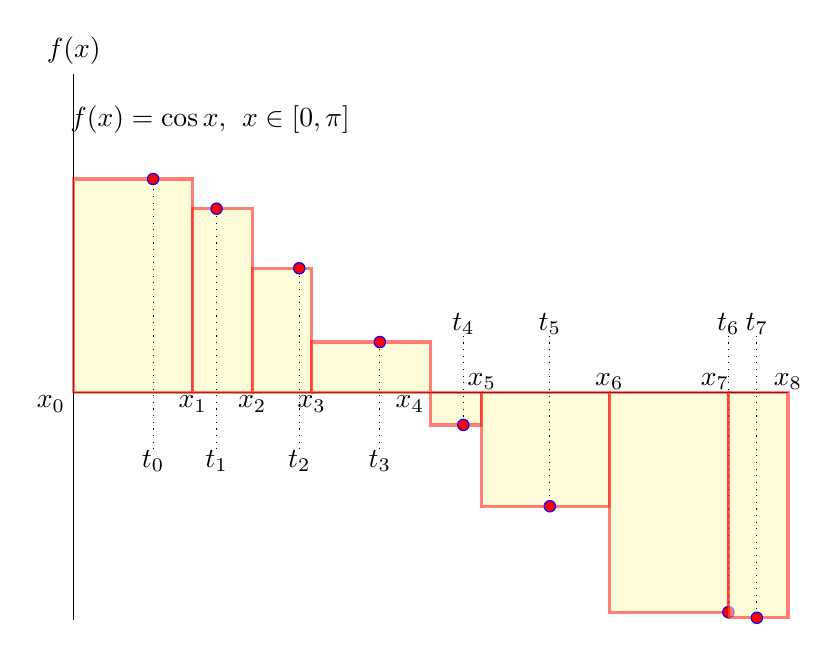
\begin{tikzpicture}[scale=\textwidth/4.2cm]
    % title and axes
    \node at (0.6, 1.2) {$f(x)=\cos x, \hspace{4pt} x \in [0, \pi]$};
    \draw (0, 0) -- (pi, 0);
    \draw (0, 0) -- (0, 1.4)
        node[above] {$f(x)$};
    \draw (0, 0) -- (0, -1);
    % graph
    \draw[black, very thick] plot[smooth] file {integrals_of_functions/python_generated_tables/cos_0_pi_riemann_sum.table};
    \draw[red, very thick, fill=yellow!30, opacity=0.5] (0, 0) 
        -- (pi/6, 0)
        -- (pi/6, {cos(pi/9 r)})
        -- (0, {cos(pi/9 r)})
        -- (0, 0);
    \node at (-0.1, -0.05) {$x_{0}$};
    \node at (pi/9, -0.3) {$t_{0}$};
    \node at (pi/6, -0.05) {$x_{1}$};
    \draw[black, dotted] (pi/9, -0.25) -- (pi/9, {cos(pi/9 r)});
    \draw[blue, fill=red] (pi/9, {cos(pi/9 r)}) circle (.25mm);
    \draw[red, very thick, fill=yellow!30, opacity=0.5] (pi/6, 0) 
        -- (pi/4, 0)
        -- (pi/4, {cos(pi/5 r)})
        -- (pi/6, {cos(pi/5 r)})
        -- (pi/6, 0);
    \node at (pi/5, -0.3) {$t_{1}$};
    \node at (pi/4, -0.05) {$x_{2}$};
    \draw[black, dotted] (pi/5, -0.25) -- (pi/5, {cos(pi/5 r)});
    \draw[blue, fill=red] (pi/5, {cos(pi/5 r)}) circle (.25mm);
    \draw[red, very thick, fill=yellow!30, opacity=0.5] (pi/4, 0) 
        -- (pi/3, 0)
        -- (pi/3, {cos(12*pi/38 r)})
        -- (pi/4, {cos(12*pi/38 r)})
        -- (pi/4, 0);
    \node at (12*pi/38, -0.3) {$t_{2}$};
    \node at (pi/3, -0.05) {$x_{3}$};
    \draw[black, dotted] (12*pi/38, -0.25) -- (12*pi/38, {cos(12*pi/38 r)});
    \draw[blue, fill=red] (12*pi/38, {cos(12*pi/38 r)}) circle (.25mm);
    \draw[red, very thick, fill=yellow!30, opacity=0.5] (pi/3, 0) 
        -- (pi/2, 0)
        -- (pi/2, {cos(12*pi/28 r)})
        -- (pi/3, {cos(12*pi/28 r)})
        -- (pi/3, 0);
    \node at (12*pi/28, -0.3) {$t_{3}$};
    \node at (8*pi/17, -0.05) {$x_{4}$};
    \draw[black, dotted] (12*pi/28, -0.25) -- (12*pi/28, {cos(12*pi/28 r)});
    \draw[blue, fill=red] (12*pi/28, {cos(12*pi/28 r)}) circle (.25mm);
    \draw[red, very thick, fill=yellow!30, opacity=0.5] (pi/2, 0) 
        -- (4*pi/7, 0)
        -- (4*pi/7, {cos(6*pi/11 r)})
        -- (pi/2, {cos(6*pi/11 r)})
        -- (pi/2, 0);
    \node at (6*pi/11, 0.3) {$t_{4}$};
    \node at (4*pi/7, 0.05) {$x_{5}$};
    \draw[black, dotted] (6*pi/11, 0.25) -- (6*pi/11, {cos(6*pi/11 r)});
    \draw[blue, fill=red] (6*pi/11, {cos(6*pi/11 r)}) circle (.25mm);
    \draw[red, very thick, fill=yellow!30, opacity=0.5] (4*pi/7, 0) 
        -- (3*pi/4, 0)
        -- (3*pi/4, {cos(2*pi/3 r)})
        -- (4*pi/7, {cos(2*pi/3 r)})
        -- (4*pi/7, 0);
    \node at (2*pi/3, 0.3) {$t_{5}$};
    \node at (3*pi/4, 0.05) {$x_{6}$};
    \draw[black, dotted] (2*pi/3, 0.25) -- (2*pi/3, {cos(2*pi/3 r)});
    \draw[blue, fill=red] (2*pi/3, {cos(2*pi/3 r)}) circle (.25mm);
    \draw[red, very thick, fill=yellow!30, opacity=0.5] (3*pi/4, 0) 
        -- (11*pi/12, 0)
        -- (11*pi/12, {cos(11*pi/12 r)})
        -- (3*pi/4, {cos(11*pi/12 r)})
        -- (3*pi/4, 0);
    \node at (11*pi/12, 0.3) {$t_{6}$};
    \node at (44*pi/49, 0.05) {$x_{7}$};
    \draw[black, dotted] (11*pi/12, 0.25) -- (11*pi/12, {cos(11*pi/12 r)});
    \draw[blue, fill=red] (11*pi/12, {cos(11*pi/12 r)}) circle (.25mm);
    \draw[red, very thick, fill=yellow!30, opacity=0.5] (11*pi/12, 0) 
        -- (pi, 0)
        -- (pi, {cos(22*pi/23 r)})
        -- (11*pi/12, {cos(22*pi/23 r)})
        -- (11*pi/12, 0);
    \node at (22*pi/23, 0.3) {$t_{7}$};
    \node at (pi, 0.05) {$x_{8}$};
    \draw[black, dotted] (22*pi/23, 0.25) -- (22*pi/23, {cos(22*pi/23 r)});
    \draw[blue, fill=red] (22*pi/23, {cos(22*pi/23 r)}) circle (.25mm);
\end{tikzpicture}
}
\begin{align*}
    &\text{The approximation can be computed with} \hspace{20pt} \sum_{i=0}^{7} f(t_{i})(x_{i+1} - x_{i})
\end{align*}
Taking a partition with uncountable infinitely many points between $0$ and $1$ is the key to computing the integral. The rectangles seen in this example each have an area: base times height. The difference $(x_{i+1} - x_{i})$ for each $i$ represents the base, while the function value at $t_{i}$ for each $i$ represents the height. So, the integral of our function $f$ ---the value of which we will discuss shortly--- can be expressed as the limit 
\begin{align*}
    \lim_{n \longrightarrow \infty} \sum_{i=0}^{n-1} \cos(t_{i}) (x_{i+1} - x_{i}) = \int_{0}^{1} \cos x dx = \sin x \hspace{4pt} x \in [0, 1]
\end{align*}
\label{integral_of_cosine}
\end{example}

\begin{theorem}
A function $f$ continuous on $[a, b]$ or continuous at all but a finite number of points along $[a, b]$ is integrable on $[a, b]$.
\label{monotone_continuous_functions_are_integrable}
\end{theorem}

Integration on the continuous functions mentioned in Theorem \ref{monotone_continuous_functions_are_integrable} will more times than not require us to use something referred to as antidifferentiation, as opposed to the computation of sums, using a result known as The Fundamental Theorem of Calculus, which we will get to later. For now, let's simply practice antidifferentiation on continuous functions and explore some properties of the Riemann integral. 

\begin{example}
The function $f(x) = \cos x$ is continuous on $[0, 1]$. Thus, for Example \ref{integral_of_cosine}, the antiderivative of $f$ is $g(x) = \sin x$.
\end{example}

\begin{example}
Take $f(x) = 1$ on some arbitrary domain $D$. The form of the integral on $f$ along this non-explicitly defined domain $D$ is referred to as the indefinite form of the integral. Meaning, the function domain is not bounded above or below by any specific real numbers. We will later discuss the difference between this indefinite form and what is known as the definite form of an integral, which we used in Example \ref{integral_of_cosine}. The domain is explicitly defined and bounded for cosine in that example, whereas the domain for $f$ in this example is not defined at all. More on this, later. In taking either form of the integral on a function $f$, the first question you should always ask yourself:
\begin{align*}
    &\text{The derivative of which function $g$ is equal to} \hspace{4pt} f?\\[2ex]
    &\text{Meaning, what is $g$, when} \hspace{4pt} \dfrac{dg}{dx} = f(x) \hspace{4pt} \text{?}
\end{align*}
Once you find $g$, \textbf{THAT} is the integral of $f$. With the indefinite form, we must consider the crucial detail of a real number (constant) as being part of the expression for our function $g$. Particularly, for our example, we know
\begin{align*}
f(x) = 1 \hspace{20pt} f(x) = 1 + 0
\end{align*}
and we know that the derivative of a constant is $0$ and the derivative of $x$ is $1$. So, when searching for the indefinite integral $g$, we not only must consider the `kernel' (the main part) of the function $f$, which in our case is $1$, we must also consider the implied $0$. 
Continuing with our example:
\begin{align*}
    \text{we know that} \hspace{20pt} \dfrac{d}{dx} (x+c) = \dfrac{d}{dx} x + \dfrac{d}{dx} c = 1 + 0 = 1 \hspace{20pt} \text{where} \hspace{4pt} c \in \mathbb{R}
\end{align*}
So, we have that $g(x) = x+c$, because $\dfrac{dg}{dx} = \dfrac{d}{dx}(x+c) = 1 + 0 = 1 = f(x)$. Additionally, because $f$ is continuous on $D$, we call $g$ an antiderivative of $f$. Thus, we have the indefinite integral
\begin{align*}
    g(x) = \int_{D} f(x)dx = \int_{D} 1 dx = x + c \hspace{20pt} \text{where $D$ is the domain of the function}
\end{align*}
which also happens to be an antiderivative. We could represent this integral without the $1$ under the integral sign, as follows
\begin{align*}
    g(x) = \int_{D} dx = x+c
\end{align*}
\end{example}

\begin{example}
Let's take the integral of $f(x) = x$. We know 
\begin{align*}
    \dfrac{d}{dx} \Big(\dfrac{x^{2}}{2} + c \Big) = \dfrac{d}{dx} \dfrac{x^{2}}{2} + \dfrac{d}{dx} c = \dfrac{2x}{2} + 0 = x
\end{align*}
So, $g(x) = \dfrac{x^{2}}{2} + c$ is the indefinite integral of $f$ and it also happens to be an antiderivative of $f$, since $f$ is continuous on $D$. The results are summarized below.
\begin{align*}
    \int_{D} f(x)dx = \int_{D} x dx  =  \dfrac{x^{2}}{2} + c = g(x)
\end{align*}
\end{example}

\begin{exercise}
Find the indefinite integral of the following
\begin{align*}
    f(x) = x^{n} \hspace{20pt} \text{where $n$ is a positive number} 
\end{align*}
\end{exercise}

\begin{exercise}
Find the indefinite integral of the following
\begin{align*}
    f(x) = x^{-n} \hspace{20pt} \text{where $n$ is a positive number}
\end{align*}
\end{exercise}

\begin{exercise}
Find the indefinite integral of the following
\begin{align*}
    f(x) = e^{x}
\end{align*}
\end{exercise}

\begin{exercise}
Find the indefinite integral of the following
\begin{align*}
    f(x) = \cos x
\end{align*}
\end{exercise}

\begin{exercise}
Find the indefinite integral of the following
\begin{align*}
    f(x) = \sin x
\end{align*}
\end{exercise}

\begin{theorem}
Following are some of the basic properties of the Riemann integral
\begin{align*}
    &\int_{D} c f(x) dx = c \int_{D} f(x) dx \hspace{20pt} \text{where} \hspace{4pt} c \in \mathbb{R}\\[2ex]
    &\int_{D} (f(x) + g(x)) dx = \int_{D} f(x) dx + \int_{D} g(x) dx\\[2ex]
    &\int_{D} (f(x) - g(x)) dx = \int_{D} f(x) dx - \int_{D} g(x) dx\\[2ex]
    &\text{If} \hspace{4pt} f(x) \geq 0 \hspace{4pt} \text{for all $x \in D$} \hspace{20pt} \text{then} \hspace{20pt} \int_{D} f(x) dx \geq 0\\[2ex]
    &\text{If} \hspace{4pt} f(x) \leq g(x) \hspace{4pt} \text{for all $x \in D$} \hspace{20pt} \text{then} \hspace{20pt} \int_{D} f(x) dx \leq \int_{D} g(x) dx
\end{align*}
\end{theorem}

\begin{exercise}
Find the indefinite integral of the following
\begin{align*}
    f(x) = 1 + 3x
\end{align*}
\end{exercise}

\begin{exercise}
Find the indefinite integral of the following
\begin{align*}
    f(x) = x^{2} + 2x - 5
\end{align*}
\end{exercise}

\begin{exercise}
Find the indefinite integral of the following
\begin{align*}
    f(x) = 2 - x^{2}
\end{align*}
\end{exercise}

\begin{exercise}
Find the indefinite integral of the following
\begin{align*}
    f(x) = 1 + 2x^{3}
\end{align*}
\end{exercise}

\begin{exercise}
Find the indefinite integral of the following
\begin{align*}
    f(x) = \dfrac{1}{2}x - 1
\end{align*}
\end{exercise}

\begin{exercise}
Find the indefinite integral of the following
\begin{align*}
    f(x) = 3 - 2x
\end{align*}
\end{exercise}

\newpage
\section{The Fundamental Theorem of Calculus}

\begin{theorem}
For function $f$ as described in Theorem \ref{monotone_continuous_functions_are_integrable}, we have the indefinite integral of $f$ represented as
\begin{align*}
    g(x) = \int_{a}^{x} f(t) dt \hspace{20pt} x \in [a, b]
\end{align*}
where $a$ is referred to as a basepoint. On the interval $[a, b]$, we have $g$ is continuous, and on the interval $(a, b)$, save for possibly finitely many points, we have $g$ is differentiable, with
\begin{align*}
    g^{'}(z) = f(z) \hspace{20pt} \text{for all} \hspace{4pt} z \in (a, b) \hspace{20pt} \text{save possibly finitely many points where $f$ is discontinuous}
\end{align*}
We refer to this as The Fundamental Theorem of Calculus I.\\[1ex]
When $f$ is continuous on the domain $[a, b]$, we call $g$ an antidervative of $f$. \label{FTC_1}
\end{theorem}

\begin{theorem}
For function $f$ as described in Theorem \ref{monotone_continuous_functions_are_integrable}, we have 
\begin{align*}
    g(b) - g(a) = \int_{a}^{b} f(x) dx \hspace{20pt} x \in [a, b]
\end{align*}
where $g$ is continuous on $[a, b]$. Also, $g$ is differentiable on $(a, b)$, save for finitely many points, with
\begin{align*}
    g^{'}(x) = f(x) \hspace{20pt} \text{for all} \hspace{4pt} x \in (a, b) \hspace{20pt} \text{save for possibly finitely many points where $f$ is discontinuous}
\end{align*}
We refer to this as The Fundamental Theorem of Calculus II.\\[1ex]
When $f$ is continuous on $[a, b]$, $g$ is an antiderivative of $f$.
\end{theorem}

\begin{exercise}
Find the definite integral of the following
\begin{align*}
    f(x) = 1 + 3x \hspace{20pt} x \in [-1, 5]
\end{align*}
\end{exercise}

\begin{exercise}
Find the definite integral of the following
\begin{align*}
    f(x) = x^{2} + 2x - 5 \hspace{20pt} x \in [1, 4]
\end{align*}
\end{exercise}

\begin{exercise}
Find the definite integral of the following
\begin{align*}
    f(x) = 2 - x^{2} \hspace{20pt} x \in [0, 2]
\end{align*}
\end{exercise}

\begin{exercise}
Find the definite integral of the following
\begin{align*}
    f(x) = 1 + 2x^{3} \hspace{20pt} x \in [0, 5]
\end{align*}
\end{exercise}

\begin{exercise}
Find the definite integral of the following
\begin{align*}
    f(x) = \dfrac{1}{2}x - 1 \hspace{20pt} x \in [0, 3]
\end{align*}
\end{exercise}

\begin{exercise}
Find the definite integral of the following
\begin{align*}
    f(x) = 3 - 2x \hspace{20pt} x \in [-1, 3]
\end{align*}
\end{exercise}

\begin{theorem}
Following are more of the basic properties of the Riemann integral
\begin{align*}
    &\text{If} \hspace{4pt} f(x) \geq 0 \hspace{4pt} \text{for all $x \in D$} \hspace{20pt} \text{then} \hspace{20pt} \int_{D} f(x) dx \geq 0\\[2ex]
    &\text{If} \hspace{4pt} f(x) \leq g(x) \hspace{4pt} \text{for all $x \in D$} \hspace{20pt} \text{then} \hspace{20pt} \int_{D} f(x) dx \leq \int_{D} g(x) dx 
\end{align*}
\end{theorem}

\begin{example}
In many situations, we could make use of a substitution method to simplify our process of integration. Take the following
\begin{align*}
    f(x) = \sqrt{2x + 1} \hspace{20pt} x \in [0, 4]
\end{align*}
We have the definite integral represented as 
\begin{align*}
    g(x) = \int_{0}^{4} \sqrt{2x + 1} dx
\end{align*}
To make the job of integration easier, we could set $u(x) = 2x + 1$. This would imply the following
\begin{align*}
    \dfrac{du}{dx} = 2 \hspace{10pt} \Longleftrightarrow \hspace{10pt} \dfrac{du}{2} = dx \hspace{20pt} \text{and} \hspace{20pt} u(x) \in [1, 9]
\end{align*}
Thus, the integral can be rewritten from this substitution as
\begin{align*}
    g(x) = \int_{1}^{9} \dfrac{1}{2}\sqrt{u(x)} du = \int_{1}^{9} \dfrac{1}{2} \hspace{4pt} (u(x))^{1/2} \hspace{4pt} du = \dfrac{1}{3} (u(x))^{3/2} \hspace{20pt} u(x) \in [1, 9]
\end{align*}
The right hand side of the equality evaluates to $26/3$. However, if one wishes to revert back to expressions in terms of $x$, as opposed to $u(x)$, the numerically computation will be the same.
\begin{align*}
    g(x) &= \int_{1}^{9} \dfrac{1}{2}\sqrt{u(x)} du = \dfrac{1}{3} (u(x))^{3/2} \hspace{20pt} u(x) \in [1, 9]\\[2ex]
    &= \dfrac{1}{3} (\sqrt{2x + 1})^{3/2} \hspace{20pt} x \in [0, 4]\\[2ex]
    &= \dfrac{1}{3} (\sqrt{2(4) + 1})^{3/2} - \dfrac{1}{3} (\sqrt{2(0) + 1})^{3/2} = \dfrac{26}{3}
\end{align*}
\end{example}

\begin{example}
Consider the following indefinite integral
\begin{align*}
    g(x) = \int_{D} \cos^{3} x \sin x dx
\end{align*}
It looks tough, but with a tool referred to as \textbf{U-Substitution}, we got this. Define
\begin{align*}
    u(x) = \cos x
\end{align*}
By differentiating $u$ with respect to $x$, we get
\begin{align*}
    \dfrac{du}{dx} = -\sin x \hspace{20pt} \Longleftrightarrow \hspace{20pt} -du = \sin x dx
\end{align*}
Thus, our indefinitie integral becomes
\begin{align*}
    g(x) &= \int_{D} -(u(x))^{3} du\\[2ex]
    &= \hspace{4pt} -\dfrac{1}{4} (u(x))^{4} + c\\[2ex]
    &= \hspace{4pt} -\dfrac{1}{4} \cos^{4} x + c
\end{align*}
\end{example}

\begin{exercise}
Find the indefinite integral of the following 
\begin{align*}
    f(x) = \dfrac{\sec^{2} \Big(\dfrac{1}{x}\Big)}{x^{2}}
\end{align*}
\end{exercise}

\begin{exercise}
Find the indefinite integral of the following 
\begin{align*}
    f(x) = x \sin(x^{2})
\end{align*}
\end{exercise}

\begin{exercise}
Find the indefinite integral of the following 
\begin{align*}
    f(x) = \dfrac{x}{(x^{2} + 1)^{2}}
\end{align*}
\end{exercise}

\begin{exercise}
Find the indefinite integral of the following 
\begin{align*}
    f(x) = e^{x} \sin (e^{x})
\end{align*}
\end{exercise}

\begin{exercise}
Find the indefinite integral of the following 
\begin{align*}
    f(x) = \dfrac{x}{x^{2} + 1}
\end{align*}
\end{exercise}

\begin{exercise}
Find the indefinite integral of the following 
\begin{align*}
    f(x) = \dfrac{(\ln x)^{2}}{x}
\end{align*}
\end{exercise}

\begin{exercise}
Find the indefinite integral of the following 
\begin{align*}
    f(x) = (1 + \tan x)^{5} \sec^{2} x
\end{align*}
\end{exercise}

\begin{exercise}
Find the indefinite integral of the following 
\begin{align*}
    f(x) = e^{x} \sin (e^{x})
\end{align*}
\end{exercise}

\begin{exercise}
Find the indefinite integral of the following 
\begin{align*}
    f(x) = \dfrac{\sin(\ln x)}{x}
\end{align*}
\end{exercise}

\begin{exercise}
Find the indefinite integral of the following 
\begin{align*}
    f(x) = \dfrac{\cos x}{\sin^{2} x}
\end{align*}
\end{exercise}

\begin{exercise}
Find the indefinite integral of the following 
\begin{align*}
    f(x) = \sqrt{\cot x} \csc^{2} x
\end{align*}
\end{exercise}

\begin{exercise}
Find the indefinite integral of the following 
\begin{align*}
    f(x) = \sec^{3} x \tan x
\end{align*}
\end{exercise}

\begin{exercise}
Find the indefinite integral of the following 
\begin{align*}
    f(x) = \dfrac{1+x}{1 + x^{2}}
\end{align*}
\end{exercise}

\begin{exercise}
Find the indefinite integral of the following 
\begin{align*}
    f(x) = \dfrac{x^{2}}{\sqrt{1 - x}}
\end{align*}
\end{exercise}

\begin{exercise}
Find the indefinite integral of the following 
\begin{align*}
    f(x) = \dfrac{x}{\sqrt[\leftroot{2}\uproot{2}4]{x + 2}}
\end{align*}
\end{exercise}

\begin{exercise}
Find the indefinite integral of the following 
\begin{align*}
    f(x) = x^{3} \sqrt{x^{2} + 1}
\end{align*}
\end{exercise}

\begin{exercise}
Find the definite integral of the following 
\begin{align*}
    f(x) = x^{2} (1 + 2x^{3})^{5} \hspace{20pt} x \in [0, 1]
\end{align*}
\end{exercise}

\begin{exercise}
Find the definite integral of the following 
\begin{align*}
    f(x) = \dfrac{e^{1/x}}{x^{2}} \hspace{20pt} x \in [1, 2]
\end{align*}
\end{exercise}

\begin{exercise}
Find the indefinite integral of the following
\begin{align*}
    f(x) = \tan x
\end{align*}
\end{exercise}

\begin{exercise}
Find the indefinite integral of the following
\begin{align*}
    f(x) = \sec x
\end{align*}
\end{exercise}

\begin{example}
Using Theorem \ref{FTC_1}, we can find the derivative of an indefinite integral. Take the following
\begin{align*}
    \int_{1}^{x^{4}} \sec t dt
\end{align*}
The function under the integral sign is continuous. Additionally, we have $x^{4}$ as our upper bound on the integral sign. Let's define $u(x) = x^{4}$. Our function $g$ can now be written as 
\begin{align*}
    g(x) = (v \circ u)(x) = \int_{1}^{u(x)} \sec t dt
\end{align*}
By The Fundamental Theorem of Calculus I, along with The Chain Rule 
\begin{align*}
    \dfrac{dg}{dx} &= v^{'}(u(x)) \cdot u^{'}(x)\\[2ex] 
    &= \dfrac{d}{du} \Big( \int_{1}^{u(x)} \sec t dt \Big) \dfrac{du}{dx}\\[2ex]
    &= ( \sec u(x) ) \cdot 4x^{3}\\[2ex]
    &= 4x^{3} \sec x^{4} 
\end{align*}
\end{example}

\begin{exercise}
Find the derivative of $g$.
\begin{align*}
    g(x) = \int_{1}^{x} \dfrac{1}{t^{3} + 1} dt
\end{align*}
\end{exercise}

\begin{exercise}
Find the derivative of $g$.
\begin{align*}
    g(x) = \int_{2}^{x} t^{2} \sin t dt
\end{align*}
\end{exercise}

\begin{note}
\begin{align*}
    \int_{b}^{a} f(x) dx = -\int_{a}^{b} f(x) dx \hspace{20pt} a, b \in \mathbb{R}
\end{align*}
\end{note}

\begin{exercise}
Find the derivative of $g$.
\begin{align*}
    g(x) = \int_{x}^{\pi} \sqrt{1 + \sec t} dt
\end{align*}
\end{exercise}

\begin{exercise}
Find the derivative of $g$.
\begin{align*}
    g(x) = \int_{2}^{1/x} \arctan t dt
\end{align*}
\end{exercise}

\begin{exercise}
Find the derivative of $g$.
\begin{align*}
    g(x) = \int_{1}^{\cos x} (1 + t^{2})^{10} dt
\end{align*}
\end{exercise}

\begin{exercise}
Find the derivative of $g$.
\begin{align*}
    g(x) = \int_{e^{x}}^{0} \sin^{3} t dt
\end{align*}
\end{exercise}

\newpage
\section{Integration by Parts}

\begin{theorem}
Let $u$, $v$ be differentiable on $[a, b]$ and let $f = u^{'}$ and $g = v^{'}$ be Riemann integrable. Then the following holds
\begin{align*}
    \int_{a}^{b} ug = uv \Big|_{a}^{b} - \int_{a}^{b} vf
\end{align*}
\begin{proof}
By the product rule
\begin{align*}
    (uv)^{'} = fv + ug = vf + ug
\end{align*}
We know differentiable functions are Riemann integrable, and we are told that $f$ and $g$ are integrable. Thus,
\begin{align*}
    \int_{a}^{b} (uv)^{'} &= \int_{a}^{b} vf + \int_{a}^{b} ug\\[2ex]
    &\Longleftrightarrow\\[2ex]
    uv \Big|_{a}^{b} &= \int_{a}^{b} vf + \int_{a}^{b} ug\\[2ex] 
    &\Longleftrightarrow\\[2ex]
    \int_{a}^{b} ug &= uv \Big|_{a}^{b} - \int_{a}^{b} vf\\[2ex]
    \int_{a}^{b} u dv &= uv \Big|_{a}^{b} - \int_{a}^{b} v du
\end{align*}
\end{proof}
We refer to this integration technique as Integration by Parts.
\end{theorem}

\begin{example}
We find the following integral
\begin{align*}
    \int_{D} \ln x dx
\end{align*}
by defining the following
\begin{align*}
    &u(x) = \ln x \hspace{20pt} \Longrightarrow \hspace{20pt} \dfrac{du}{dx} = \dfrac{1}{x} \hspace{20pt} \Longleftrightarrow \hspace{20pt} du = \dfrac{dx}{x}\\[2ex]
    &dv = dx \hspace{20pt} \Longrightarrow \hspace{20pt} v(x) = \int_{D} dv = \int_{D} dx = x
\end{align*}
Using Integration by Parts, with $c_{0}, c_{1} \in \mathbb{R}$ this gives us the following setup
\begin{align*}
    \int_{D} \ln x dx = \int_{D} u(x) dv = u(x)v(x) - \int_{D} v(x) du = \ln x \cdot x + c_{0} - \int_{D} x \dfrac{dx}{x} = \ln x \cdot x + c_{0} - x + c_{1}
\end{align*}
We now combine our constants into one constant $c$ for the final result
\begin{align*}
    \int_{D} \ln x dx = x \ln x - x + c
\end{align*}
\end{example}

\begin{exercise}
Find the indefinite integral of the following
\begin{align*}
    f(x) = x^{2} \ln x
\end{align*}
\end{exercise}

\begin{exercise}
Find the indefinite integral of the following
\begin{align*}
    f(x) = x \cos x
\end{align*}
\end{exercise}

\begin{exercise}
Find the indefinite integral of the following
\begin{align*}
    f(x) = x \cos(mx) \hspace{20pt} m \in \mathbb{R}
\end{align*}
\end{exercise}

\begin{exercise}
Find the indefinite integral of the following
\begin{align*}
    f(x) = x^{2} e^{x}
\end{align*}
\end{exercise}

\begin{exercise}
Find the indefinite integral of the following
\begin{align*}
    f(x) = \sin x \cdot e^{x}
\end{align*}
\end{exercise}

\begin{exercise}
Find the indefinite integral of the following
\begin{align*}
    f(x) = \arctan x
\end{align*}
\end{exercise}

\begin{exercise}
Find the indefinite integral of the following
\begin{align*}
    f(x) = x \sec^{2} x
\end{align*}
\end{exercise}

\begin{exercise}
Find the indefinite integral of the following
\begin{align*}
    f(x) = x \cdot 2^{x}
\end{align*}
\end{exercise}

\begin{exercise}
Find the indefinite integral of the following
\begin{align*}
    f(x) = e^{-x} \cos(2x)
\end{align*}
\end{exercise}

\begin{exercise}
Find the definite integral of the following
\begin{align*}
    f(x) = \dfrac{\ln x}{x^{2}} \hspace{20pt} x \in [1, 2]
\end{align*}
\end{exercise}

\begin{exercise}
Find the definite integral of the following
\begin{align*}
    f(x) = \dfrac{x}{e^{2x}} \hspace{20pt} [0, 1]
\end{align*}
\end{exercise}

\begin{exercise}
Find the definite integral of the following
\begin{align*}
    f(x) = \arccos x \hspace{20pt} \Big[0, \hspace{4pt} \dfrac{1}{2}\Big]
\end{align*}
\end{exercise}

\begin{note}
There are times when multiple integration approaches/techniques make integration easier.
\end{note}

\begin{exercise}
Find the indefinite integral of the following
\begin{align*}
    f(x) = x^{3} \cos(x^{2}) \hspace{20pt} \Big[\sqrt{\dfrac{\pi}{2}}, \hspace{4pt} \sqrt{\pi} \Big]
\end{align*}
\end{exercise}

\begin{exercise}
Find the definite integral of the following
\begin{align*}
    f(x) = e^{\cos x} \sin(2x) \hspace{20pt} [0, \pi]
\end{align*}
\end{exercise}

\begin{exercise}
Find the indefinite integral of the following
\begin{align*}
    f(x) = \cos \sqrt{x}
\end{align*}
\end{exercise}

\newpage
\section{Trigonometric Integrals}

\begin{recall}
We will use the following trigonometric identities, along with previously discussed techniques, to solve the integrals within this section.
\begin{align*}
    &1 = \cos^{2} x + \sin^{2} x\\[2ex]
    &\cos(2x) = \cos^{2} x - \sin^{2} x\\[2ex]
    &\sin(2x) = 2\sin x \cos x
\end{align*}
\end{recall}

\begin{exercise}
Find the definite integral of the following
\begin{align*}
    f(x) = \cos x \hspace{20pt} x \in \Big[0, \hspace{4pt} \dfrac{\pi}{2} \Big]
\end{align*}
\end{exercise}

\begin{exercise}
Find the definite integral of the following
\begin{align*}
    f(x) = \sin^{2}(2x) \hspace{20pt} x \in \Big[0, \hspace{4pt} \dfrac{\pi}{2} \Big]
\end{align*}
\end{exercise}

\begin{exercise}
Find the indefinite integral of the following
\begin{align*}
    f(x) = \sin^{3} x \cos^{2} x
\end{align*}
\end{exercise}

\begin{exercise}
Find the definite integral of the following
\begin{align*}
    f(x) = \sin^{2} x \cos^{2} x \hspace{20pt} x \in \Big[0, \dfrac{\pi}{2} \Big]
\end{align*}
\end{exercise}

\begin{exercise}
Find the indefinite integral of the following
\begin{align*}
    f(x) = x \cos^{2} x
\end{align*}
\end{exercise}

\begin{exercise}
Find the indefinite integral of the following
\begin{align*}
    f(x) = \sec^{2} x \tan x
\end{align*}
\end{exercise}

\begin{exercise}
Find the indefinite integral of the following
\begin{align*}
    f(x) = \tan^{2} x 
\end{align*}
\end{exercise}

\begin{exercise}
Find the definite integral of the following
\begin{align*}
    f(x) = \sec^{4} x \tan^{4} x \hspace{20pt} x \in \Big[0, \dfrac{\pi}{4} \Big]
\end{align*}
\end{exercise}

\begin{exercise}
Find the indefinite integral of the following
\begin{align*}
    f(x) = \tan^{3} x \sec x
\end{align*}
\end{exercise}

\begin{exercise}
Find the indefinite integral of the following
\begin{align*}
    f(x) = \dfrac{\sin x}{\cos^{3} x}
\end{align*}
\end{exercise}

\begin{exercise}
Find the definite integral of the following
\begin{align*}
    f(x) = \cot^{2} x \hspace{20pt} \Big[\dfrac{\pi}{6}, \dfrac{\pi}{2}\Big]
\end{align*}
\end{exercise}

\begin{exercise}
Find the indefinite integral of the following
\begin{align*}
    f(x) = \csc x
\end{align*}
\end{exercise}

\begin{exercise}
Find the definite integral of the following
\begin{align*}
    f(x) = \csc^{3} x \hspace{20pt} \Big[\dfrac{\pi}{6}, \dfrac{\pi}{3}\Big]
\end{align*}
\end{exercise}

\newpage
\section{Integration by Partial Fractions}

\begin{recall}
We call the quotient of two polynomials a rational function. Let $p$ and $q$ be polynomials. Then $r$, with the following definition, is a rational function
\begin{align*}
    r(x) = \dfrac{p(x)}{q(x)}
\end{align*}
In this section, we will deal with rational functions, some of which may require long division. Following are a few details about which forms of rational functions we are likely to encounter within this section, as well as some examples of how to break these forms down into partial fractions that are relatively easier to integrate.
\end{recall}

\begin{note}
The rational functions that we will deal with in this section may include within their denominators some of the following:
\begin{itemize}
    \item Distinct, linear factors
    \item Non-distinct, linear factors
    \item Distinct, irreducible, quadratic factors
    \item Non-distinct, irreducible, quadratic factors
\end{itemize}
\label{four_cases_for_partial_fractions}
\end{note}

\begin{recall}
Long division of polynomials takes place when the degree of the polynomial in the denominator is less than the degree of the polynomial in the numerator.
\end{recall}

\begin{example}
Let
\begin{align*}
    f(x) = \dfrac{x^{3} + x}{x - 1}
\end{align*}
Using an algorithm for long division of polynomials
\begin{align*}
\setstackgap{S}{1.5pt}
\stackMath\def\stackalignment{r}
\stackunder{
  x-1 \stackon[1pt]{\showdiv{x^{3} + \hspace{20pt} + x}}{x^{2} + x + 2}
}{
  \Shortstack[l]{{\underline{x^{3}-x^{2}}\ph{\hspace{10pt} + x}} \ph{x^{3}-}x^{2}+x {\ph{x^{3}-}\underline{x^{2}-x}} \ph{x^{3}-x^{2}-}2x {\ph{x^{3}-x^{2}-}\underline{2x}} 
   \ph{x^{3}-x^{2}-}0}
  }
\end{align*}
Thus,
\begin{align*}
    f(x) = \dfrac{x^{3} + x}{x - 1} = x^{2} + x + 2 + \dfrac{0}{x - 1} = x^{2} + x + 2
\end{align*}
\end{example}

\begin{example}
We wish to integrate the following function
\begin{align*}
    f(x) = \dfrac{x^{2} + 2x - 1}{2x^{3} + 3x^{2} - 2x}
\end{align*}
Our goal is to rewrite this rational function in one of the four forms mentioned in Note \ref{four_cases_for_partial_fractions}. Factoring the denominator, we get
\begin{align*}
    \dfrac{x^{2} + 2x - 1}{2x^{3} + 3x^{2} - 2x} = \dfrac{x^{2} + 2x - 1}{x(2x - 1)(x + 2)}
\end{align*}
We see that each linear factor in the denominator. We may now break the single fraction into multiple fractions, as follows
\begin{align*}
    \dfrac{x^{2} + 2x - 1}{x(2x - 1)(x + 2)} = \dfrac{a}{x} + \dfrac{b}{2x - 1} + \dfrac{c}{x + 2}
\end{align*}
Multiplying through by the factored denominator, we have
\begin{align*}
    (x(2x - 1)(x + 2)) \cdot \dfrac{x^{2} + 2x - 1}{x(2x - 1)(x + 2)} \hspace{4pt} &= \hspace{4pt} (x(2x - 1)(x + 2)) \cdot \Big(\dfrac{a}{x} + \dfrac{b}{2x - 1} + \dfrac{c}{x + 2} \Big)\\[2ex]
    &\Longleftrightarrow\\[2ex]
    x^{2} + 2x - 1 \hspace{4pt} &= \hspace{4pt} a(2x - 1)(x + 2) + bx(x + 2) + cx(2x - 1)
\end{align*}
After a bit of rearrangement, we get
\begin{align*}
    x^{2} + 2x - 1 \hspace{4pt} = (2a + b + 2c)x^{2} + (3a + 2b - c)x - 2a
\end{align*}
Now, we can set the coefficients for the polynomial on the left-hand side equal to the coefficients for the polynomial on the right-hand side
\begin{align*}
    1 &= 2a + b + 2c\\[2ex]
    2 &= 3a + 2b - c\\[2ex]
    -1 &= -2a
\end{align*}
Using our experience with systems of equations, we get
\begin{align*}
    a = \dfrac{1}{2} \hspace{20pt} b = \dfrac{1}{5} \hspace{20pt} c = -\dfrac{1}{10}
\end{align*}
giving us the resulting integral
\begin{align*}
    \int_{D} \dfrac{x^{2} + 2x - 1}{2x^{3} + 3x^{2} - 2x} dx &= \int_{D} \Big(\dfrac{1}{2} \cdot \dfrac{1}{x} + \dfrac{1}{5} \cdot \dfrac{1}{2x - 1} - \dfrac{1}{10} \cdot \dfrac{1}{x + 2}\Big) dx\\[2ex]
    &= \dfrac{1}{2}\int_{D} \dfrac{1}{x} dx \hspace{4pt} + \hspace{4pt} \dfrac{1}{5}\int_{D} \dfrac{1}{2x - 1} dx \hspace{4pt} - \hspace{4pt} \dfrac{1}{10}\int_{D} \dfrac{1}{x+2} dx\\[2ex]
    &= \dfrac{1}{2}\ln \lvert x \rvert + \dfrac{1}{10}\ln \lvert 2x - 1 \rvert - \dfrac{1}{10}\ln \lvert x + 2 \rvert + k
\end{align*}
where $k \in \mathbb{R}$
\end{example}

\begin{example}
The general form resulting from the breakdown of rational functions with (exclusively) distinct linear factors within the denominator is as follows
\begin{align*}
    f(x) = \frac{p(x)}{q(x)} &= \dfrac{p(x)}{(a_{1}x + b_{1})(a_{2}x + b_{2}) \cdots (a_{n-1}x + b_{n-1})(a_{n}x + b_{n})}\\[2ex]
    &= \dfrac{c_{1}}{a_{1}x + b_{1}} + \dfrac{c_{2}}{a_{2}x + b_{2}} + \cdots + \dfrac{c_{n-1}}{a_{n-1}x + b_{n-1}} + \dfrac{c_{n}}{a_{n}x + b_{n}}
\end{align*}
\end{example}

\begin{example}
As an example of how we may break a rational function, the denominator of which containing repeating linear factors, down into multiple partial fractions, take
\begin{align*}
    f(x) = \dfrac{x^{4} - 2x^{2} + 4x + 1}{x^{3} - x^{2} - x + 1}
\end{align*}
Using long division, we can rewrite $f$ as follows
\begin{align*}
    f(x) = \dfrac{x^{4} - 2x^{2} + 4x + 1}{x^{3} - x^{2} - x + 1} = x + 1 + \dfrac{4x}{x^{3} - x^{2} - x + 1}
\end{align*}
Factoring the denominator of the resulting fractional portion of the rational function, we get
\begin{align*}
    f(x) = x + 1 + \dfrac{4x}{x^{3} - x^{2} - x + 1} = x + 1 + \dfrac{4x}{(x-1)^{2} (x+1)}
\end{align*}
Breaking this down to partial fractions, noting that $(x-1)$ occurs twice, we get
\begin{align*}
    f(x) = x + 1 + \dfrac{4x}{(x-1)^{2} (x+1)} = x + 1 + \dfrac{a}{x - 1} + \dfrac{b}{(x - 1)^{2}} + \dfrac{c}{x + 1}
\end{align*}
\end{example}

\begin{example}
The general form resulting from the breakdown of rational functions with (exclusively) repeating linear factors within the denominator is as follows
\begin{align*}
    f(x) = \dfrac{p(x)}{q(x)} &= \dfrac{p(x)}{(ax + b)^{n}}\\[2ex]
    &= \dfrac{c_{1}}{(ax + b)} + \dfrac{c_{2}}{(ax + b)^{2}} + \cdots \dfrac{c_{n-1}}{(ax + b)^{n-1}} + \dfrac{c_{n}}{(ax + b)^{n}}
\end{align*}
\end{example}

\begin{example}
As an example of how to break a rational function, the denominator of which containing irreducible quadratic factors, down into multiple partial functions, take
\begin{align*}
    f(x) = \dfrac{x}{(x-2)(x^{2} + 1)(x^{2} + 4)}
\end{align*}
We can now take the function $f$ and rewrite it as multiple rationals, each with a single factor in its denominator
\begin{align*}
    f(x) &= \dfrac{x}{(x-2)(x^{2} + 1)(x^{2} + 4)}\\[2ex]
    &= \dfrac{a}{x-2} + \dfrac{bx + c}{x^{2} + 1} + \dfrac{dx + e}{x^{2} + 4}
\end{align*}
\end{example}

\begin{example}
The general form resulting from the breakdown of rational functions with (exclusively) distinct, irreducible quadratic factors within the denominator is as follows
\begin{align*}
    f(x) = \dfrac{p(x)}{q(x)} &= \dfrac{p(x)}{(a_{1}x^{2} + b_{1}x + c_{1}) \cdots (a_{n}x^{2} + b_{n}x + c)}\\[2ex]
    &= \dfrac{d_{1}x + e_{1}}{a_{1}x^{2} + b_{1}x + c_{1}} + \cdots + \dfrac{d_{n}x + e_{n}}{a_{n}x^{2} + b_{n}x + c_{n}}
\end{align*}
\end{example}

\begin{example}
As an example of how to break a rational function, the denominator of which containing repeating, irreducible quadratic factors, down into multiple partial functions, take
\begin{align*}
    f(x) = \dfrac{x^{3} + x^{2} + 1}{x(x-1)(x^{2} + x + 1)(x^{2} + 1)^{3}}
\end{align*}
We can now take the function $f$ and rewrite it as multiple rationals, each with a single factor in its denominator
\begin{align*}
    f(x) &= \dfrac{x^{3} + x^{2} + 1}{x(x-1)(x^{2} + x + 1)(x^{2} + 1)^{3}}\\[2ex]
    &= \dfrac{a}{x} + \dfrac{b}{x-1} + \dfrac{cx + d}{x^{2} + x + 1} + \dfrac{ex + f}{x^{2} + 1} + \dfrac{gx + h}{(x^{2} + 1)^{2}} + \dfrac{ux + v}{(x^{2} + 1)^{3}}
\end{align*}
\end{example}

\begin{example}
The general form resulting from the breakdown of rational functions with (exclusively) repeating, irreducible quadratic factors within the denominator is as follows
\begin{align*}
    f(x) &= \dfrac{p(x)}{q(x)} = \dfrac{p(x)}{(ax^{2} + bx + c)^{n}}\\[2ex]
    &= \dfrac{c_{1}x + d_{1}}{ax^{2} + bx + c} + \dfrac{c_{2}x + d_{2}}{(ax^{2} + bx + c)^{2}} + \cdots + \dfrac{c_{n-1}x + d_{n-1}}{(ax^{2} + bx + c)^{n-1}} + \dfrac{c_{n}x + d_{n}}{(ax^{2} + bx + c)^{n}}
\end{align*}
\end{example}

\begin{exercise}
Find the indefinite integral of the following
\begin{align*}
    f(x) = \dfrac{x}{x-6}
\end{align*}
\end{exercise}

\begin{exercise}
Find the indefinite integral of the following
\begin{align*}
    f(x) = \dfrac{1}{(x+4)(x-1)}
\end{align*}
\end{exercise}

\begin{exercise}
Find the definite integral of the following
\begin{align*}
    f(x) = \dfrac{1}{x^{2} - 1} \hspace{20pt} x \in [2, 3]
\end{align*}
\end{exercise}

\begin{exercise}
Find the definite integral of the following
\begin{align*}
    f(x) = \dfrac{x^{3} - 4x - 10}{x^{2} - x - 6} \hspace{20pt} x \in [0, 1]
\end{align*}
\end{exercise}

\begin{exercise}
Find the indefinite integral of the following
\begin{align*}
    f(x) = \dfrac{1}{(x+5)^{2} (x-1)}
\end{align*}
\end{exercise}

\begin{exercise}
Find the indefinite integral of the following
\begin{align*}
    f(x) = \dfrac{1}{x^{2} (x - 1)^{2}}
\end{align*}
\end{exercise}

\begin{exercise}
Find the indefinite integral of the following
\begin{align*}
    f(x) = \dfrac{x^{3} + 4}{x^{2} + 4}
\end{align*}
\end{exercise}

\begin{exercise}
Find the indefinite integral of the following
\begin{align*}
    f(x) = \dfrac{x^{2} + x + 1}{(x^{2} + 1)^{2}}
\end{align*}
\end{exercise}

\begin{exercise}
Find the indefinite integral of the following
\begin{align*}
    f(x) = \dfrac{x + 4}{x^{2} + 2x + 5}
\end{align*}
\end{exercise}

\begin{exercise}
Find the definite integral of the following
\begin{align*}
    f(x) = \dfrac{x}{x^{2} + 4x + 13} \hspace{20pt} x \in [0, 1]
\end{align*}
\end{exercise}

\newpage
\section{Improper Integrals}

\begin{theorem}
For functions that follow the structure
\begin{align*}
    f(x) = \dfrac{1}{x^{p}} \hspace{20pt} x \in [1, \infty)
\end{align*}
we have the following
\begin{align*}
    \int_{1}^{\infty} \dfrac{1}{x^{p}} dx
\end{align*}
is convergent for $p > 1$ and divergent for $p \leq 1$
\end{theorem}

\begin{example}
Take $f(x) = \dfrac{1}{x}$ from $[1, \infty)$. We set up the integral as follows
\begin{align*}
    \int_{1}^{\infty} \dfrac{1}{x} dx
\end{align*}
and then replace the $\infty$ in the upper bound with a variable, say $b$, and push that variable to $\infty$ as follows
\begin{align*}
    \int_{1}^{\infty} \dfrac{1}{x} dx = \lim_{b \longrightarrow \infty} \int_{1}^{b} \dfrac{1}{x} dx
\end{align*}
Now, we can evaluate using the Fundamental Theorem of Calculus, per usual
\begin{align*}
    \lim_{b \longrightarrow \infty} \int_{1}^{b} \dfrac{1}{x} dx &= \lim_{b \longrightarrow \infty} (\ln x) \Big|_{1}^{b}\\[2ex]
    &= \lim_{b \longrightarrow \infty} \ln b - \ln 1 
\end{align*}
As you can see, when $b \longrightarrow \infty$, the integral pushes to infinity. 
\end{example}

\newpage
\section{Series of Numbers}

Geometric\\
Integral Test\\
Comparison Tests\\
Alternating Series\\
Ratio, Root Tests\\



\newpage
\section{Bibliography}

\begin{thebibliography}{9}
\bibitem{undergraduate_analysis_bartle}
Bartle, Robert G., Sherbert, Donald R.; \textit{Introduction to Real Analysis}; $4^{\text{th}}$ ed.;\\ John Wiley and Sons, Inc.

\bibitem{stewart_calculus}
Stewart, James; \textit{Calculus Early Transcendentals}; $6^{\text{th}}$ ed.;\\ Thomson Learning, Inc.

\bibitem{undergraduate_analysis_rudin}
Rudin, Walter; \textit{Principles of Mathematical Analysis}; $2^{\text{nd}}$ ed.;\\ McGraw Hill Book Company

\bibitem{undergraduate_analysis_stoll}
Stoll, Manfred; \textit{Introduction to Real Analysis}; $2^{\text{nd}}$ ed.;\\ Addison-Wesley Higher Mathematics

\bibitem{statistical_inference}
Casella, George; Berger, Roger L; \textit{Statistical Inference}; $2^{\text{nd}}$ ed.;\\ Duxbury Thomson Learning

\end{thebibliography}

\end{document}
